\documentclass[a4paper, 11pt]{article}

\usepackage{amsmath}
\usepackage{graphics}
\usepackage{epsfig}
%\usepackage{ipe} 
\usepackage{latexsym}
\usepackage{amssymb}
\usepackage{color}
%\usepackage{here}
\usepackage{url}
     
\parindent 0pt
\parskip 3mm

\setlength{\textwidth}{18cm}
\setlength{\evensidemargin}{-1cm}
\setlength{\oddsidemargin}{-1cm}

\newcommand{\bblue}[1]{{\color{blue} #1}}
\newcommand{\rred}[1]{{\color{red} #1}}
\newcommand{\ggreen}[1]{{\color{green} #1}}
      
\newcommand{\svsp}{\vspace{3mm}}
\newcommand{\vsp}{\vspace{5mm}}
\newcommand{\bvsp}{\vspace{10mm}}
\newcommand{\ind}{\mbox{}\hspace{2cm}}
\newcommand{\sind}{\mbox{}\hspace{1cm}}
      
\newcommand{\B}{\condmath{I\!\!B}}    
\newcommand{\D}{\mathbb D}              
\newcommand{\E}{\mathbb E}            
\newcommand{\F}{\mathbb F}            
%\newcommand{\Id}{\condmath{I\!\!I}}                  
\newcommand{\I}{\mathbb I}
\newcommand{\M}{\mathbb M}
\newcommand{\N}{\mathbb N}
\newcommand{\Q}{\mathbb Q}
\newcommand{\R}{\mathbb R}
\renewcommand{\S}{\mathbb S}
\newcommand{\Z}{\mathbb Z}


\newcommand{\aaa}{\condmath{\cal A}}            
\newcommand{\cc}{\condmath{\cal C}} 
\newcommand{\e}{\condmath{\varepsilon}}   
\newcommand{\lcal}{{\condmath{\cal L}}      }
\newcommand{\mm}{{\condmath{\cal M}}      }
\newcommand{\pp}{\condmath{{\cal P}}}
\newcommand{\sss}{{\condmath{\cal S}}}
\newcommand{\vv}{\condmath{\cal V}}            
\newcommand{\tc}{\condmath{\cal T}}   

%\newcommand{\+}{{\footnotesize +}}   
\newcommand{\+}{\mbox{{\tiny +}}}   
      
\newcommand{\aff}{{\rm aff}}
\newcommand{\aire}{{\rm aire}}
\newcommand{\area}{\operatorname{area}}
\newcommand{\bis}{{\rm bis}}
\newcommand{\conv}{{\rm conv}}
%\newcommand{\degre}{{\rm deg}}
\newcommand{\del}{{\rm Del}} 
\newcommand{\dels}{\del _{\sss}(E)}
\newcommand{\delc}{{\rm DelC}}     
\newcommand{\dist}{\mbox {dist}}  
\newcommand{\dom}{{\rm dom}}
\newcommand{\insphere}{{\tt in\_sphere}}
\newcommand{\inter}{{\rm int}}
\newcommand{\intd}{\int\!\!\int}  %integrale multiple
\newcommand{\lag}{{\rm Lag}}
\newcommand{\length}{\operatorname{length}}
\newcommand{\lfs}{{\rm lfs}}
\newcommand{\lift}{{\rm lift}}
\newcommand{\ma}{\condmath{\cal M}}
\newcommand{\norm}[1]{\| #1 \|}
\newcommand{\obj}{{\condmath{\cal O}}}
\newcommand{\orient}{{\tt orient}}
\newcommand{\para}{{\condmath{\cal Q}}}
\newcommand{\plan}{P}
\newcommand{\ppv}{{\rm ppv}}
\newcommand{\point}{{\rm point}}
\newcommand{\power}{{\tt power\_test}}
\newcommand{\proba}{{\rm proba}}
% \newcommand{\proj}{\mbox {proj}} 
\newcommand{\proj}{\pi_S} 
\newcommand{\pts}{E}
\newcommand{\rch}{{\rm rch}}
\newcommand{\sign}{{\rm sign}}
\newcommand{\str}{{\rm star}}
\newcommand{\surf}{{\condmath{\cal S}}}
\newcommand{\sym}{{\rm sym}}
\newcommand{\tub}{\mbox {tube}}
\newcommand{\thk}{\mbox {thick}}
\newcommand{\vect}[1]{\,\overrightarrow{#1}}
\newcommand{\vol}{{\rm vol}}
\newcommand{\vor}{{\rm Vor}}
\newcommand{\voro}{Vorono�}
\newcommand{\vors}{\vor _{\sss}(E)}
\newcommand{\wfs}{{\rm wfs}}
\newcommand{\wit}{{\rm Wit}}
\newcommand{\suwit}{{\rm SuWit}}
            
\newcommand{\ceil}[1]{\left\lceil #1 \right\rceil}
\newcommand{\floor}[1]{\left\lfloor #1 \right\rfloor}
\newcommand{\bin}[2]{\, \left( \begin{array}{c} #1 \\ #2 \end{array} \! \right)} 
\renewcommand{\v}[1]{{\bf #1}} %vectors
     
\newcommand{\determinant}[4]{\, \left| \begin{array}{cc} #1 & #2 \\ #3 & #4 \end{array} \! \right|}
\newcommand{\Det}[3]{\, \left| \begin{array}{c} #1 \\ #2 \\ #3 \end{array} \! \right|}
\newcommand{\Determinant}[9]{\, \left| \begin{array}{ccc} #1 & #2 & #3 \\ #4 & #5 & #6 \\ #7 & #8 & #9 \end{array} \! \right|}
\def\condmath#1{\leavevmode\ifmmode #1 \else $#1$ \fi}

\newenvironment{proof}
        {\noindent \textbf{Proof.} \hspace{0.3mm}}
        {\hspace{0.3mm}$\square$  \smallskip}      
     
\newcommand{\JPdraw}[1]{
                \begin{figure}[h]
                \begin{center} \input{#1.ltex} \end{center}
                \end{figure}
                }
      
%\newenvironment{proof_e}
%        {\noindent \textbf{Proof.} \hspace{0.3mm}}
%        {\hspace{0.3mm}$\square$  \smallskip}      
     

\pagestyle{headings}

\newtheorem{theorem}{Theorem}
\newtheorem{Theorem}{Theorem}      
\newtheorem{claim}{Claim}
\newtheorem{corol}{Corollary}
\newtheorem{Corol}{Corollary}
\newtheorem{corollary}{Corollary}
\newtheorem{defin}{Definition}
\newtheorem{definition}{Definition}
\newtheorem{fact}{Fact}
\newtheorem{Fact}{Fact}
\newtheorem{lem}{Lemma} 
\newtheorem{lemma}{Lemma}
\newtheorem{observation}{Observation}
\newtheorem{property}{Property}
\newtheorem{Property}{Property}
\newtheorem{proposition}{Proposition}
\newtheorem{prop}{Proposition}    
\newtheorem{question}{Exercise}
\newtheorem{questions}{Exercises}
\newtheorem{quest}{Question}
\newtheorem{remark}{Remark}  



\newcommand{\cqfd}{\mbox{}\hfill $\Box$ \medskip}

\parindent 0pt
\parskip 2mm



\usepackage{amsmath}
\usepackage{latexsym}
\usepackage{amssymb}
\usepackage{url}

\setlength{\textwidth}{18cm}
\setlength{\evensidemargin}{-1cm}
\setlength{\oddsidemargin}{-1cm}

\pagestyle{myheadings}
\markright{J-D. Boissonnat\ \ \ \ \ \ \ \ \ \ \ \ \ \ \ \ \ \ \ \ \ \ \ \ \ \ \ 
  \ \ \ \ \ \ \ \ \ \ \ \ \ \ GUDHI  \ \ \ \ \ \ \ \ \ \ \ \ \ \ \ \ \
  \ \ \ \ \ \ \ \ \ \ \ \ \ \ \ \ \ \ \ Part B1}

\parindent 0pt
\parskip 0.7mm

\begin{document}
\thispagestyle{empty}

\mbox{}\vspace{-3.5cm}

\begin{center}
{\Large
{\bf ERC Advanced Grant 2012 \\ research proposal (PART B1)}}
\vspace{6mm}

{\LARGE {\bf  Algorithmic Foundations \\ of 
Geometry Understanding in Higher Dimensions}

\vspace{2mm} 

{\bf (GUDHI)}
}
\end{center}

\vspace{3mm}

\begin{tabbing}
Name of PI~:  \hspace{1.9cm} \=  Jean-Daniel Boissonnat\\
Host Institution : \> INRIA\\
Proposal full title : \> Algorithmic Foundations of 
Geometry Understanding  in Higher Dimensions\\ 
Proposal short name : \> GUDHI \\
Proposal duration : \> 60 months
\end{tabbing}

\vspace{-3mm}

% \begin{document}
% \thispagestyle{empty}

% \mbox{}\vspace{-3.5cm}

% \begin{center}
% {\Large
% {\bf ERC Advanced Grant 2012 \\ research proposal (PART B1)}}
% \vspace{1cm}

% {\LARGE {\bf  Algorithmic Foundations \\ of 
% Geometry Understanding in Higher Dimensions}

% \vspace{3mm} 

% {\bf (GUDHI)}
% }
% \end{center}

% \vspace{4mm}

% \begin{tabbing}
% Name of PI~:  \hspace{1.9cm} \=  Jean-Daniel Boissonnat\\
% Host Institution : \> INRIA\\
% Proposal full title : \> Algorithmic Foundations of 
% Geometry Understanding  in Higher Dimensions\\ 
% Proposal short name : \> GUDHI \\
% Proposal duration : \> 60 months
% \end{tabbing}

% \vspace{2mm}

% -*- LaTeX -*-

%\begin{abstract}
 %  After sound, images and videos, 3D models are everywhere and used for multimedia, video games, numerical simulations, manufacturing, computer-aided medicine, culturage heritage and other fields. In parallel to this new multimedia revolution during the past decade, exceptional progress was made in elaborating the theoretical and algorithmic foundations of 3D geometric modeling, and providing efficient algorithms and codes for applications such as surface reconstruction, mesh generation and point cloud processing.  Extending those techniques to higher dimensions is a grand challenge with a huge potential impact in science and engineering but is currently extremely limited and asks for new algorithmic  breakthrough. This project aims at settling the algorithmic foundations of geometric modeling in higher dimensions and to propose a well-principled ground-breaking software platform allowing technological advances for varied applications in science and engineering.


\paragraph{Proposal summary.} 

% <<<<<<< .mine
% =======
% The need for computer-aided {\em understanding} of geometric structures, geometry understanding for short, is ubiquitous in science and has become an essential part of {\em scientific computing} and {\em data analysis}. Geometry understanding is by no means limited to three dimensions and many applications in physics, biology, and engineering require a keen understanding of the geometry of a variety of higher dimensional spaces. Let us mention phase space in particle physics, invariant manifolds in dynamical systems, configuration spaces of mechanical systems, conformational spaces of molecules, image manifolds, and shape spaces, to name a few. In {\em data analysis and manifold learning}, data are often thought as points in some high-dimensional metric space. Those points are usually not uniformly distributed in the embedding space but lie close to some {\em low-dimensional manifold}, which reflects the fact that the physical system that produced the data has a moderate number of degrees of freedom.  Understanding the geometry of this manifold is key to understanding the underlying system. We do not refer to a single action: the term geometry understanding encompasses a collection of tasks including representing and approximating the manifold, extracting the manifold from the point set, and inferring some geometric or topological properties.
% >>>>>>> .r121

The central goal of this proposal is to settle the algorithmic
foundations of geometry understanding in dimensions higher than 3.  We
coin the term {\em geometry understanding} to encompass a collection
of tasks including the computer representation and the approximation
of geometric structures, and the inference of geometric or topological
properties of sampled
shapes.  % geometric structure from point sets.

The need to understand geometric structures is ubiquitous in science
and has become an essential part of {\em scientific computing} and
{\em data analysis}. %In {\em scientific computing},
Geometry understanding is by no means limited to
three dimensions and many applications in physics, biology, and
engineering require a keen understanding of the geometry of a variety
of {\em higher dimensional spaces}. Let us mention phase space in particle
physics, invariant manifolds in dynamical systems, configuration
spaces of mechanical systems, conformational spaces of molecules,
image manifolds, and shape spaces, to name a few.  {\em Data
  analysis} is a major area where understanding
geometry in high dimensional spaces is  needed to
 capture concise information from the underlying structure of
 data. Our approach is complementary to {\em manifold learning}
 techniques and aims at  developing an effective theory for {\em geometric and
 topological data analysis.}
% The central focus of this proposal is the computer analysis of
% geometric structures, which we refer to as {\em geometry
%   understanding}.  The need for analyzing geometric structures is
% ubiquitous in science and has become an essential part of {\em scientific
% computing and data analysis}. Geometry understanding is by no means
% limited to 3-dimensions and many applications in physics, biology and
% engineering require a keen understanding of the geometry of a variety
% of higher dimensional spaces. Let us mention phase space in particle
% physics, invariant manifolds in dynamical systems, configuration
% spaces of mechanical systems, conformational spaces of molecules,
% image manifolds, or shape spaces.
% Data analysis  is another place where understanding
% geometry in high-dimensional spaces is needed to
% capture concise information from the underlying structure of the data.  
% Since data are produced at an unprecedented rate in all
% sciences, understanding the geometry of high-dimensional data %point clouds
% has become a core task in science and engineering.

The central goal of this proposal is to settle the {\em algorithmic
  foundations} of geometry understanding in {\em dimensions higher
  than 3}.  We intend to develop {\em scalable representations} in the
form of {\em simplicial complexes}, and {\em practical algorithms} to
approximate highly nonlinear shapes, and to infer geometric and
topological properties from data subject to significant {\em defects}
and under {\em realistic conditions}.  As is common in many
applications across science and engineering, we will assume that the
objects of interest can be modeled as {\em low-dimensional manifolds}
embedded in possibly high-dimensional spaces. By exploiting the {\em
  intrinsic properties} of the objects, we will produce intrinsic
dimension-sensitive data structures and algorithms that will break the
current computational bottleneck.

To reach these objectives, the guiding principle will be to foster a
symbiotic relationship between theory and practice, and to address
{\em fundamental research} issues along three parallel advancing
fronts. We will simultaneously develop {\em mathematical approaches}
providing theoretical guarantees, {\em effective algorithms} that are
amenable to theoretical analysis and rigorous experimental validation,
and {\em perennial software} development.  We will undertake the
development of a high-quality open source {\em software platform} to
implement the most important geometric data structures and algorithms
at the heart of geometry understanding in higher dimensions. The
platform will be a unique vehicle towards researchers from other
fields and will serve as a {\em basis for groundbreaking advances} in
scientific computing and data analysis.


%\vspace{-3mm}

\paragraph{Keywords :} Computational geometry, computational topology,
manifold learning, homology inference, simplicial complexes,
scientific computing, data analysis


\newpage

% \paragraph{A cultural note.}
% A gudhi is found hanging out of a window or otherwise
% prominently displayed in traditional Maharashtrian households. Gudhi is
% a bright green or yellow cloth adorned with brocade (zari) tied to the
% tip of a long bamboo over which gathi (sugar crystals), neem
% leaves, a twig of mango leaves and a garland of red
% flowers is tied. A silver or copper pot is placed in the inverted
% position over it. This gudhi is then hoisted outside the house, in a
% window, terrace or a high place so that everybody can see it.

% Some of the significances attributed to raising a Gudhi are as follows:

%  --   Gudhi symbolizes the Brahmadhvaj (translation: Brahma’s flag)
%     mentioned in the Brahma Purana, because Lord Brahma created the
%     universe on this day. It may also represent Indradhvaj
%     (translation: the flag of Indra).

% --   Mythologically, the Gudhi symbolizes Lord Rama’s victory and
%    happiness on returning to Ayodhya after slaying Ravan. Since a symbol
%    of victory is always held high, so is the gudhi (flag). It is believed
%    that this festival is celebrated to commemorate the coronation of Rama
%    post his return to Ayodhya after completing 14 years of exile.

% --    Maharashtrians also see the Gudhi as a symbol of victory
%     associated with the conquests of the Maratha forces led by
%     Chhatrapati Shivaji. It also symbolizes the victory of King
%     Shalivahana over Sakas and was hoisted by his people when he
%     returned to Paithan. Gudhi is believed to ward off evil, invite
%     prosperity and good luck into the house.


%\newpage

\section{The principal investigator}

\subsection{Curriculum Vitae}

I was born in Nice, May 18, 1953. I am married and have 3 children. I am a french citizen.

\paragraph{Education}\mbox{}

$\bullet$ I graduated from the Ecole Sup\'erieure d'Electricit\'e (Sup\'elec) in 1976.  Sup\'elec is among the top ``Grandes Ecoles'' in France and the reference in the field of electric energy and information sciences. Sup\'elec is on a par with the best departments of electrical and computer engineering of the top American or European universities.
$\bullet$
I obtained my PhD Thesis in Information Theory from the University of Rennes (1979). 
$\bullet$
I obtained the Habilitation diploma (the highest grade at french universities) in Computer Science from the  University of Nice in 1992.

\paragraph{Professional academic experience}\mbox{}

 $\bullet$ I have been a researcher at INRIA since 1980, first in Rocquencourt and since 1986 in Sophia Antipolis.  $\bullet$  I am currently a {\em Research Director} (on par with full professor) at INRIA Sophia-Antipolis (France) where I lead the Geometrica research group. I was promoted in 2009 at the highest rank (Exceptional Class) for my contributions to research, formation and dissemination. $\bullet$ I held important positions within INRIA. I have been 
the {\em VP for Science}  at INRIA Sophia-Antipolis (500 employees, 38 research groups) (2001-2005). 
I have also been  the {\em chairman of the Evaluation Committee} of the institute, one of the most eminent positions at INRIA with a key role in the definition and the implementation
of the scientific policy of the institute (2005-2009).  This position gave me  a comprehensive view of the research performed in the eight research centers of INRIA.


% \paragraph{Scientific expertise} \mbox{}
% Computational Geometry, Algorithmic Robotics, Geometric Computing, Mesh Generation, Shape Reconstruction, Geometric Learning

\paragraph{Scientific leadership} \mbox{}

% I conducted My {\em scientific research} is mainly in computational geometry and topology, geometric modeling, algorithmic robotics and medical imaging.
% My main {\em contributions} are on  mesh generation, surface reconstruction, motion planning, robust geometric computing, randomized algorithms, Voronoi diagrams, Delaunay triangulations, manifold learning,  and to a lower extent on structural biology and control theory.

My first research group at INRIA, {\em Prisme}, has been the birth place of Computational Geometry in France and played a prominent role in shaping the field~\cite{by-ag-98}. 
I contributed and directed research on Voronoi diagrams, Delaunay triangulations, randomized algorithms, motion planning, exact computing, and, most importantly, initiated 15 years ago the development of the {\em CGAL library} in collaboration with partners in Europe (\url{http://www.cgal.org}{}).

In 2003, I founded the {\em Geometrica} research group in replacement of Prisme. The main objective was to develop Nonlinear Computational Geometry. 
 Geometrica's research in this area has been flourishing and well regarded internationally. Together with my students and collaborators, I made seminal contributions on mesh generation and surface reconstruction (see ref. 1-2, 5, 7-8 in Section~\ref{trackrecord}). A very visible output of this research has been the development of CGAL components. These components are now used worldwide in academia and in industry for various applications in geometric modeling, medical imaging and geology.\footnote{see \url{http://www-sop.inria.fr/geometrica/software/cgalmesh/}}

Together with F. Chazal, we established in 2006 a subgroup of Geometrica in {\em Saclay} (Paris's area)  to strengthen our work on  the emerging field of {\em geometric inference}.  This resulted in influential contributions to the analysis of distance functions, persistent homology, manifold learning and the development of geometric inference~\cite{geometrica-7142i,ccsm-gipm-2011}
\newpage


\paragraph{Publications and patents} \mbox{}

I am the author of over 150 technical publications including 1 text book, 57 journal articles, 91 refereed international conference articles, 12 book chapters.  I edited 4 books. My {\em h-number is 47 with 7786 citations} according to Google Scholar. 

I am the author of {\em 4 patents}~: 2 on mesh generation (Assignee: Institut Francais du P\'etrole (IFP)), robotic surgery (Assignee: Intuitive Surgical Inc.), virtual endoscopy (Assignee: Siemens Corporate Research)).

\paragraph{Software} \mbox{}

I am the author of two software that have been commercialized at large scale by major companies, one by Siemens (Flying Through, installed on Siemens scanners) and one by Dassault Systems (integrated in Catia V5 (Shape Editor)). 

My research group Geometrica has been one of the leader teams of  the CGAL Open Source Project since its start (\url{http://www.cgal.org}{}).  The CGAL library  is now regarded as the {\em gold standard in Computational Geometry} with a huge impact, both in academia and in industry.\footnote{For a few identified academic projects using CGAL (including two ERC Starting Grant projects), see
\url{http://www.cgal.org/projects.html}} Notably, the triangulation package of CGAL, developed within Geometrica, is now integrated in the heart of Matlab.

\paragraph{Supervision of Ph.D. students, postdocs and young researchers} \mbox{}

I have supervised 24 Ph.D. students. All of them are enjoying successful careers in academia or industry. I am currently advising two Ph.D. students. One of my former students, Andreas Fabri, founded in 2003 GeometryFactory, a startup company that commercializes CGAL.

Three members of my research group successfully  created their own research groups at INRIA with varied topics~: J-P. Merlet (Robotics), F. Cazals (Structural Biology), S. Lazard (Computational Geometry). Another member of the group, P. Alliez (who received an ERC starting grant), is in the process of creating his own group on geometry processing and modeling of urban scenes.

\paragraph{Academic awards and honors}\mbox{}

$\bullet$ I received two highly prestigious prizes, the {\em IBM award in Computer Science}  in 1987
and the {\em Grand prize EADS in Information Sciences} in 2006 (awarded by the {\em French Academy of Science}).  $\bullet$  I was nominated to the {\em international Roberval prize} for the french version of my book ”Algorithmic Geometry” coauthored by M. Yvinec (The Roverval prize awards the best scientific textbook in french). $\bullet$  I have been received in the {\em National Order of Merit} (Order of State awarded by the President of the French Republic)  in 2006.
My student C. Maria and I received a best paper awards at the European Symp. on Algorithms (ESA 2012).

\paragraph{Funding ID} \mbox{}

 % I have been the site leader of 8 European projects and the project leader of  the IST Project ECG ("Effective Computational Geometry") (2001-2004). % These projects gave a proeminent position to the European community of computational geometry, and led to the successful development of CGAL.

% I have been the principal investigator of 8 collaborations with french industry. The collaboration with Dassault Syst\`emes, a world leader in Geometric Modeling,  is of particular significance for this project %. We have been collaborating  with Dassault Syst\`emes for more than 10 years 
% (commercialization of software, joint publications).

We obtained with my team a budget of external funds of approximately 1.3 million Euros to support our research activities during the period 2007-2011 which divides into 0.5 from European projects,
0.5 from ANR projects (ANR is the french National Research Agency) and 0.3 from industry.

I am a site leader of the {\em ICT Fet-Open project} Computational Geometric Learning (CGL) which is closely related to the Gudhi project (\url{http://cglearning.eu/}). CGL will end in 2013. 
%http://cordis.europa.eu/fp7/ict/fet-open/) portfolio-cglearning_en.html. 

\newpage

\subsection{10-year track record}
\label{trackrecord}

\paragraph{Top 10 publications as senior researcher}  \mbox{} 

{\em Citations are according to Google Scholar. For journal articles, I added the citations of the conference version of the article. Discrete and Computational Geometry and the Symposium on Computational Geometry are regarded as the most prestigious journal and conference in Computational Geometry.}

%1. Triangulations in CGAL. Comput. Geom. Theory Appl.  Vol. 22 (2002) 5-19. Coauthors: O. Devillers, S. Pion, M. Teillaud, M. Yvinec. (26 citations including those of the conference version)

1. J-D. Boissonnat, F. Cazals. Smooth surface reconstruction via natural neighbour interpolation of
distance functions.  Comput. Geom. Theory Appl. Vol. 22 (2002) 185-203.  (421 citations)

2.  J-D. Boissonnat, F. Cazals. Natural neighbour coordinates of points on a surface.  
Comput. Geom. Theory Appl., Vol. 19, No 2-3, July 2001. (74 citations)

3. D. Attali, J-D. Boissonnat, A. Lieutier. Complexity of the Delaunay Triangulation of Points on Surfaces~: the 
Smooth Case. 20th  ACM      Symposium on Computational Geometry, 2003. 
(74 citations)

4. D. Attali, J-D. Boissonnat. A Linear Bound on the Complexity of the Delaunay Triangulation of Points on Polyhedral Surfaces.  Discrete and Comp. Geometry 31: 369--384
(2004). (61 citations)

5. J-D. Boissonnat, S. Oudot. Provably good sampling and meshing of surfaces. Graphical Models, 67 (2005) 405-451. (198 citations. Graphical Models Top-Cited Article 2005-2010)
% including those of the conference version

6. D. Attali, J-D. Boissonnat, H. Edelsbrunner. Stability and computation of medial axes~: a state-of-the-art report.
In {\em Mathematical Foundations of Scientific Visualization,
Computer Graphics, and Massive Data Exploration},
T. Moeller,   B. Hamann and B. Russell Ed.,
Springer, series Mathematics and Visualization, 2007. (93 citations)

7. J-D. Boissonnat, D. Cohen-Steiner, G. Vegter. Isotopic implicit surface meshing.  Discrete and Computational Geometry,  39: 138-157,  2008. (55 citations)% including those of the conference version)

8. J-D. Boissonnat, C. Wormser and M. Yvinec. Locally uniform anisotropic meshing. 
24th ACM Symposium on Computational Geometry, SoCG'08.
(16 citations but,  in my opinion, one of the most important papers in this list. It  led to several significant results related to the proposal, e.g.~\cite{geometrica-7142i}).

9. J-D. Boissonnat, L. Guibas, S. Oudot. Manifold reconstruction in arbitrary dimensions using witness complexes.
Discrete and Comp. Geom. Vol 42, No 1, 2009. (46 citations)

% 8. An efficient implementation of the Delaunay triangulation and
%   its graph in medium dimension.  25th ACM Symposium on Computational
%   Geometry, SoCG'09.  Coauthors: O. Devillers and S. Hornus.

10. J-D. Boissonnat, F. Nielsen, R. Nock. On Bregman Voronoi diagrams.
Discrete and Comp. Geom. (2), 2010. (76 citations)% including those of the conference version)

%10. Triangulating Smooth Submanifolds  with Light Scaffolding.
%Mathematics in Computer Science, 4(4):431-462, 2011. Coauthor: A. Ghosh.

\vspace{-1mm}

\paragraph{Edited Books and Proceedings}  \mbox{}

$\bullet$
Algorithmic Foundations of Robotics V, Springer 2004. Coeditors:  J. Burdick, 
K. Goldberg, S. Hutchinson.
$\bullet$ Effective Computational Geometry for Curves and Surfaces,
  Springer, 2006. Coeditor:  M. Teillaud. I coauthored two chapters of this book.
$\bullet$  Curves and Surfaces.
Coeditors:  P. Chenin, A. Cohen,  C. Gout, T. Lyche, M-L.  Mazure and L. Schumaker,
Springer Verlag LNCS Vol. 6920, 2012.
$\bullet$
Geometric Computing, special issue of the 
International Journal of Computational Geometry and Applications, Vol. 11, 
No. 1, 2001.
$\bullet$
Computational Geometry, Theory and Applications, Vol. 35 No. 1-2, August 2006.
Special issue on the 20th Symposium on Computational
Geometry.  %Coeditor:   J. Snoeyink.
$\bullet$ 
Discrete and Computational Geometry, Vol. 36, No 4, December 2006.
Special issue on the 20th Symposium on Computational
Geometry.  %Coeditor:   J. Snoeyink.

\vspace{-1mm}

\paragraph{Granted patents} \mbox{}

$\bullet$  Methods and apparatus for planning robotic surgery. 
United States Patent Application 20030109780. Assignee INRIA and
Intuitive Surgical Inc. (2002).  Coauthors: E. Coste-Mani\`ere, L. Adhami,
A. Carpentier, G. Guthart.
$\bullet$  Method and apparatus for fast automatic centerline extraction for virtual 
endoscopy. United States Patent Application  20050033114. Siemens Corporate 
Research (2004). Coauthor B. Geiger.

\vspace{-1mm}

\paragraph{Keynote presentations (since 2004)}\mbox{}

$\bullet$ International Symposium on Voronoi Diagrams, Tokyo (2004).
$\bullet$  Workshop "The World a Jigsaw: Tessellations in the Sciences", Leiden (2006).
$\bullet$  French Academy of Science (2 talks, 2006). 
$\bullet$  Franco Preparata's schriftfest, Brown university (2007). 
$\bullet$ Seventh conference on "Mathematical Methods for Curves and Surfaces", Toensberg, Norway, 2008. 
$\bullet$  Colloquium on Emerging Trends in Visual Computing (ETVC, Ecole Polytechnique, 2008). 
$\bullet$  22th Sibgrapi, Rio de Janeiro (2009).  
$\bullet$  ATMCS 2012 (Algebra and Topology; Methods, Computation, and Science), Edinburgh (2012).

\vspace{-1mm}

\paragraph{Membership to editorial board of international journals}   \mbox{}


I am on the editorial board of 5 international scientific journals, including two among the most prestigious  journals in Computer Science, the {\em Journal of the ACM} and  {\em Algorithmica}, and the first venue in my field {\em Discrete and Computational Geometry}. 


% I have been on the program committee of many international conferences.
% $\bullet$  {\em Algorithmica} (1990-) $\bullet$  {\em The Int. J. on Computational Geometry and Applications} (1991-)
% $\bullet$  {\em Discrete and Computational Geometry } (2006-)
% $\bullet$  {\em The Journal of Computational Geometry} (2009-)
% $\bullet$  {\em The Journal of the ACM }(2010-)

\vspace{-1mm}

\paragraph{Organization of international conferences} \mbox{}

%I have been a member of the Computational Geometry Steering Committee (1999-2001). 
%I chaired the Symposium on Computational Geometry (the top conference of the field) in 1997 and

$\bullet$ I co-chaired the program committee of the  Symposium on Computational Geometry (SCG), the top conference of the field,  in 2004. $\bullet$ I chair the Geometry Week in conjonction with SCG 2013.
$\bullet$ 
I chaired the Workshop on Algorithmic Foundations of Robotics (WAFR) in 2002.
$\bullet$ 
I have been a member of the steering committee of SCG  (1999-2001) and of the scientific committees of the International Conference on Curves and Surfaces (2010) and of  the eighth conference on "Mathematical Methods for Curves and Surfaces" (2012).
$\bullet$ 
I have been on the program committee of  the following international conferences~: Symposium on Geometry Processing (each year since its creation in 2003), 
STACS 2001 (Symposium on Theoretical Aspects of Computer Science),
ESA 2003 (European Symposium on Algorithms),
SCG'04 (Symposium on Computational Geometry)
SMI'05 (Shape Modelling International),
SMP'05 (ACM Symposium on Solid and Physical Modeling),
Curves and Surfaces 2006,
GMP 2012 (Geometric Modeling 
and Processing).

\vspace{-1mm}

\paragraph{International prizes/awards/academy memberships} \mbox{}

$\bullet$ I received the Grand prize EADS in Information Sciences in 2006 (awarded by the French Academy of Science).  $\bullet$ I received the Graphical Models Top-Cited Article for the period 2005-2010 for  my paper with S. Oudot (ref. 5 above). I received, together with my student C. Maria, one of the two best paper awards at the European Symposium on Algorithms ESA 2012~\cite{bm-dssc-2012}.

\vspace{-1mm}

\paragraph{Scientific councils and international visiting committees (2001-)} \mbox{}


$\bullet$  Scientific Council of the Ecole Normale Sup\'erieure de Lyon (2000-2003)
$\bullet$  Member of the AERES Board (French Evaluation Agency for
  Research and Higher Education)
% $\bullet$  Member of working groups 1 (Mod\`eles et calcul) and 2
%   (Logiciels et systèmes informatiques) of Allist\`ene (Alliance des sciences et technologies du num\'erique)
$\bullet$  Chair of the Visiting Committee of LIAMA, a  national center for international research of the chinese ministry of science, hosted by the Institute of Automation of the Chinese Academy of Sciences  (Beijing, 2010)
$\bullet$  Member of the Visiting Committee of the Computer Science department of ULB (Free University of Brussels, 2011)
$\bullet$    Chair of the Visiting Committee of the Geometric Modeling and Scientific Visualization  Center of the King Abdullah University of Science and Technology (KAUST, Saudi Arabia, 2012)




\newpage

\section{Extended synopsis of the project}

\paragraph{The need to understand higher-dimensional spaces and shapes}
% 3D shapes are now ubiquitous and there is no need to motivate 
%  % with applications ranging from numerical simulations, visualization, reverse engineering, and in so many fields
% % medical imaging, cultural heritage, 
% that it may be considered strange that the huge amount of techniques developed for modeling 3D
% shapes has not yet found extensions to higher dimensions. This project is built on the conviction that it is time to remedy to this state of affairs.

% Geometric modeling refers to the construction and the manipulation of computerized representations of shapes. Since shape is the first and foremost attribute of 
% our familiar 3D world, geometric modeling has been and still is a core discipline with a vast array of applications ranging from multimedia to engineering through computer-aided medicine. It has been  on the research agenda of several communities like  computer-aided design, computer graphics, computer vision, computational geometry, geometry processing and numerical analysis.

% Until now, most of the work on geometric modeling has been restricted to 3D shapes. However, 
%The need to represent higher-dimensional spaces and shapes 
is ubiquitous in science.  Physicists are used to combine space and time into a single 4-dimensional {\em space-time} continuum.  In particle physics, the {\em phase space} consists of all possible values of position and momentum variables and is 6-dimensional.  {\em Configuration spaces} of mechanical systems, {\em conformational spaces} of macromolecules are other examples of common high-dimensional geometric objects.  Although their needs may be very different, numerical simulations, motion planning, molecular docking are among celebrated applications where approximating and processing high-dimensional objects is a central issue. 

A maybe less intuitive place where one needs to understand  high-dimensional geometry is in {\em data analysis}. Natural and artificial systems like biological or sensor networks are often described by a large number of real parameters, whereas a collection of text documents can be represented as a set of term frequency vectors in Euclidean space; similar interpretations can be given for image and video data~\cite{sl-mwp-2000}.  Data analysis can then be turned into a geometric problem by encoding those heterogeneous data as clouds of points in high dimensional spaces equipped with some appropriate metric. Usually those points are not distributed in the whole embedding space but, due to the very nature of the system that produced those data, lie close to some subset of much smaller intrinsic dimension. Hence, the data conveys some geometric structure whose extraction and analysis are key to understanding the underlying system.
Since data are produced at an unprecedented rate in all sciences, 
%modeling complex high-dimensional shapes and extracting geometric information from point clouds in high-dimensional spaces have become core tasks in science and engineering. 
understanding the geometry of high-dimensional point clouds has become a core task in science and engineering. 

% The availability of tools for assisting geometric modeling and data analysis in higher-dimensional spaces may have a huge impact in applications as diverse as numerical simulations, medical imaging, bioinformatics, astrophysics and finance.


%eager need for appropriate tools that will 
% There are many other situations where complex, heteregeneous data are encoded as clouds of points in high dimension. They routinely surface in applications as diverse as medical imaging, bioinformatics, astrophysics and finance.


% A text can be considered as a point in high dimension with word frequencies acting as coordinates. Similarly, in image processing, an image of a million colorful pixels can be considered as a point in $10^6$-dimensional spaces, i.e. each pixel's RGB intensity is taken as a separate coordinate. 


% \paragraph{Unveiling the geometry of data.} {\em structure exists, conveys information, recovering this information is
% an important issue for applications : compression, analysis/learning,
% automatic processing of huge amounts of data
% Examples : images, galaxies, bio }

% In fact geometric data are ubiquitous and produced at an unprecedented rate.  They arise from measurements and simulations in the natural sciences that can easily be converted into geometric point cloud data. Most of these data reside in high-dimensional spaces.  



% An important feature of modern science and engineering is that data of various kinds is being produced at an unprecedented rate. This is so in part because of new experimental methods, and in part because of the increase in the availability of high powered computing technology. It is also clear that the nature of the data we are obtaining is significantly different. 

\paragraph{The curses of higher-dimensional geometry.} 

High-dimensional geometries are much more difficult to process and analyse than 3D shapes. The dimensionality severely restricts our intuition and ability to visualize the data. Hence  understanding higher dimensional shapes must rely on automated tools able to extract useful qualitative and quantitative information from the input high-dimensional data.

Moreover, the complexity of the data structures and of the algorithms used to  approximate shapes  rapidly grows as the dimensionality increases, which makes them intractable in high dimensions.  This curse of {\em dimensionality} is exemplified by the size of one of the simplest representations of a point set, namely its convex hull, whose complexity depends exponentially on the dimension. 
%last sentence can be removed

In addition, high-dimensional data often suffer from significant {\em defects}, including sparsity, noise, and outliers  which make them much more difficult to process than 3D data routinely provided by scanning devices. This is particularly so in the case of biological data, such as high throughput data from microarray or other sources. Moreover, the structure and occurrence of geometric features in the data may depend on the {\em scale} at which it is considered, thus requiring the analysis process to be multiscale.  

\paragraph{The emergence of computational topology.}
The last decade has seen tremendous progress in processing high-dimensional shapes and spaces. In robotics~\cite{sml-pa-2006}, randomized techniques have been proposed to capture the topology of configuration spaces and to search paths. In machine learning, a variety of techniques have been proposed to reduce the dimension of data, learn nonlinear manifolds and cluster data~\cite{hs-fmmds-2006}. In computational geometry, new approaches have been proposed to solve basic problems like searching nearest neighbours, computing smallest enclosing ellipsoids or approximating convex sets.
Most  of these methods have limited guarantees and 
%address elementary questions (which may be very hard to solve though) and 
impose strong constraints on the dimension or the topology of the shapes they can successfully handle. Computational topology emerged as a new discipline  to 
provide solid foundations for the effective understanding of complex shapes~\cite{hh-ct-2010}. 
The concepts of $\varepsilon$-samples, restricted Delaunay triangulation, anisotropic meshes emerged together with the first efficient and provably correct algorithms for emblematic problems like mesh generation and shape reconstruction in 3-dimensions~\cite{geometrica-ecg-book}. 

 The attempt to extend these results to higher dimensions led to the development of beautiful pieces of theory with deep roots in various areas of mathematics like Riemannian geometry, geometric measure theory, differential and algebraic topology. Let us mention  the emergence of a sampling theory of geometric objects and of geometric inference~\cite{geometrica-ccl09}, and the groundbreaking invention and rapid growth of persistent homology~\cite{eh-ph-2008}.
Although of a fundamental nature, these advances 
attracted  interest in several fields like data analysis, computer vision or sensor networks.

\paragraph{The computational bottleneck.}

 % Although there is a crucial need for geometric modeling tools in higher dimensions, the theoretical results obtained so far  only led to prototype codes, and applications have been limited to low dimensions or to rather crude techniques. 

%The project addresses fundamental issues in an emerging field with huge potential impact.
% it has not yet penetrated applied fields due to the lack of satisfactory algorithmic solutions in high-dimensional spaces. 
% This project is intended to remedy to this situation by proposing  a long-standing alliance between mathematical developments, algorithmic design and advanced programming.


However, the current theory has not demonstrated its scalability to real problems and, up to now, it has only been applied to rather simple cases and in low dimensions. This is  due to the lack of satisfactory algorithmic solutions in high-dimensional spaces.
Breaking the computational bottleneck is now the main issue.  Settling the {\em algorithmic foundations} of geometry understanding in
higher dimensions
%al geometric modeling 
is a grand challenge of great theoretical and practical significance. 


The tenet of this proposal is that, to take up the challenge, we need a global approach involving
tight and long-standing interactions between mathematical developments, algorithmic design and advanced programming. We believe that this is key to obtaining methods with built in
robustness, scalability and guarantees, and therefore  impact in the long run.
Such an approach has been successfully carried out in low dimensions with the 
development of the Computational Geometric Algorithms Library CGAL~\cite{cgal}. 

%We want to build upon this success 
By following this paradigm, we want  to give to  geometry understanding in higher dimensional an effective theory and a reference software platform. 
We strongly believe that this ambitious objective is realistic and can be reached. To pave the way towards this goal, we have identified  four main scientific challenges that will also correspond to the main worktasks of the project.

% \paragraph{The emerging field of structural data analysis.} {\em Early geometric approaches, 
% dimension reduction, NL manifold learning, computational topology, geometric inference
% 3d data processing, surface reconstruction, simplification. }


\paragraph{Scientific challenge 1 :  Going beyond affine models and Euclidean spaces.}

% Standard methods like PCA in Machine Learning to deal with high dimensional data assume that the data can be well approximated by some affine subspace of small dimension.  To overcome this 

In the last decades, a set of new geometric methods, known as manifold learning, have been developed with the intent of parametrizing nonlinear shapes embedded in high-dimensional spaces. Although widely used, those methods  assume very restrictive hypotheses on the geometry of the manifolds sampled by the datapoints to ensure correctness. 
A different route, inspired by what has been done in 3-dimensions, consists in approximating highly nonlinear shapes by {\em simplicial complexes}, the analogue of triangulations in higher dimensions. Recent research has exhibited sampling conditions under which  topological or geometric properties, or even a full approximation of the sampled shape can be recovered~\cite{nsw-fhm-2008,geometrica-ccl09,geometrica-7142i}. Still the sampling conditions are quite stringent, the simplicial complexes are huge objects and their construction may be problematic.  
%Progress in higher-dimensions so far has been mostly theoretical and a  huge gap  remains to be %filled before  having at one's disposal fully satisfactory solutions of practical significance.% One research direction is to invent simplicial complexes of small complexity and easy to compute that still capture the main features of the underlying shape. see Attali and Carlsson. 

A fundamental issue is the choice of a metric which determines the type and quality of an approximation.
 The simple Euclidean distance in the ambient space, while easy to deal with, is often not the right choice.  As already mentionned, most of the time, when working in high dimensional spaces, we are in fact interested by objects of much smaller intrinsic dimension. The intrinsic geometry on the objects provides the right framework. Computational intrinsic geometry has not been seriously tackled yet and a basic question like the existence of  Delaunay triangulations on Riemannian manifolds is still open.  This question is of utmost importance for anisotropic mesh generation and optimal approximations. Another important situation is when the data are not given as a point cloud in some Euclidean space, but rather as a matrix of pairwise distances (i.e. a discrete metric space). Although such data may not be sampled from geometric subsets of Riemannian manifolds, it may still carry some interesting topological structures that need to be understood. 

In information theory, signal and image processing, other pseudo-distances such as Kullback-Leibler, Itakura-Saito or Bregman divergences are preferred.  
%  In computer  vision, divergences are used throughout all the process of object recognition: to detect features using statistical, algebraic or geometric techniques, and to use these features throughout classifiers.
%The recognition of objects in potentially complex scenes is a major issue in Computer Vision. 
% Prominent advances in object recognition integrate two essential stages: the induction of features of limited size, over a potentially huge feature space, and the use of these features for learning and classification. 
These divergences are usually not true distances (they may not be symmetric nor satisfy the triangular inequality) and it is necessary to revisit geometric data structures and algorithms in this context~\cite{geometrica-6154a}.




\paragraph{Scientific challenge 2 :  Bypassing the curse of dimensionality.} 

The complexities of many geometric algorithms and data structures grow exponentially with increasing dimension. %This behavior is commonly called the curse of dimensionality after Bellman.  An immediate consequence is that it is no longer possible to partition a high dimensional space. 
This rules out most, even if not all, geometric algorithms developed in low dimensions.  Hence, extending Computational Geometry in high dimensions cannot be done in a straightforward manner and one has to take advantage of additional structure of the problem or to restrict attention to approximation. This motivated a number of new algorithmic paradigms such as locality-sensitive hashing, smoothed analysis, intrinsic algorithms.  In this project, we will address the curse of dimensionality by focusing on the inherent structure in the data which in some sense needs to be sparse or of low intrinsic dimension as well as by putting the emphasis on output-sensitive algorithms and average-case analysis~\cite{sl-mwp-2000}.  
First investigations led to very promising results, such as the design of new simplicial complexes with good complexity and approximation algorithms that scale well with the dimension \cite{cds-tewc-2004,geometrica-7142i}.


An important feature is that, even if we go to approximate solutions, we do not want to sacrifice guarantees. This is mandatory since the behaviour of algorithms in high dimensions is much less intuitive and easy to predict than in small dimensions. %\framebox{Numerics?} 





% The intrinsic geometric structure is often not easy to capture. In some situations the object is implicitly known and one can query the object of interest using appropriate oracles to get new information  (black-box model). In other situations like in Data Analysis, detecting the hidden structure is part of the problem. 

\paragraph{Scientific challenge 3 : Searching for stable models.} 
When dealing with approximation and samples, one needs stability results to ensure that the quantities that are computed are good approximations of the real ones. This is especially true in higher-dimensions where data are usually corrupted by various types of noise. A number of groundbreaking new approaches appeared recently.  {\em Topological persistence} was recently introduced as a powerful tool for the study of the topological invariants of sampled spaces~\cite{eh-ph-2008}. % Given a point cloud in Euclidean space, the approach consists in building a simplicial complex whose elements are filtered by some user-defined function. Under reasonable conditions on the input point cloud, and modulo a right choice of filter, the most persistent invariants in the filtration correspond to invariants of the space underlying the data~\cite{geometrica-cseh-07}. Thus, the persistence algorithm allow to recover global information from noisy data.

To deal with {\em non-local noise} and outliers, another  new paradigm for point cloud data analysis has emerged recently.  Point clouds are no longer treated as mere compact sets but rather as empirical measures. A notion of distance to such measures has been defined and shown to be stable with respect to perturbations of the measure \cite{ccsm-gipm-2011}. A big challenge is to find efficient algorithms in arbitrary dimensions to compute or approximate the topological structure of the sublevel-sets of the distance to a measure. Such algorithms would naturally find applications in topological inference in the presence of significant noise and outliers, but also in other less obvious contexts such as stable clustering. 

{\em Multiscale reconstruction} is another novel approach~\cite{geometrica-bgo-09}. Taking advantage of the ideas of persistence, the approach consists in building a one-parameter family of simplicial complexes approximating the input at various scales. %  It was shown that, for a sufficiently dense input data set, the family contains a long sequence of complexes that approximate the underlying space provably well, both in a topological and in a geometric sense. In fact, there can be several such sequences, each one corresponding to a plausible reconstruction at a certain scale. Thus,
 Determining the topology and shape of the original object reduces to finding the stable sequences in the one-parameter family of complexes. Despite its nice features, multiscale reconstruction, in its current form, can only be applied to low-dimensional data sets in practice. 



\paragraph{Scientific challenge 4 : Building up the reference platform for high-dimensional geometric modeling.}



% We plan to follow an integrated approach of developing the geometric foundations theoretically, but also practically in the form of high quality software on which many applications can build. With the vision of a “high-dimensional CGAL” in mind, we will develop algorithms and data structures with theoretical guarantees that should be directly applicable in Numerical Simulations, Data Analysis and and Geometric Computing, and that can serve as a basis for robust applications in fields such as Computer Vision, Medical Imaging, Robotics or Structural Biology.

% An important focus of Computational Geometry (especially of the European community) has been the design and analysis of geometric algorithms and data structures. This focus is well reflected in one of the major success stories of computational geometry, namely the Computational Geometry Algorithms Library (CGAL) that provides easy access to efficient and reliable geometric algorithms in the form of a C++ library. In most cases, reliability is achieved through guarantees.  CGAL is by now the gold standard for low dimensional geometric computing.

Software development is a central issue in this project and we will devote a substantial part of the effort to build up a software platform that will provide easy access to efficient and reliable high-dimensional geometric algorithms in the form of a C++ library. We will follow the example of the Computational Geometry Algorithms Library (CGAL), one of the major success stories of computational geometry, by now the gold standard for low dimensional geometric computing~\cite{cgal}. 
 Our project aims at extending this success story, combining efficiency with correctness guarantees to high-dimensional geometric computation.

The development of  a reference platform for high-dimensional geometric modeling is dictated by three main motivations.
{\em First}, the software platform will allow to experiment at a large scale, which is mandatory to 
design the right models and data structures. It will boost theoretical research  in geometric modeling, computational geometry in high dimensions, and computational topology, leading towards a virtuous circle between theory and experimental research. This has proven to be of utmost importance when developing the CGAL library and will be even truer in high dimensional geometry.

{\em Second}, maintaining such a platform will help further effort and consolidation in the long run.  Having a library with interoperable modules will allow to incrementally add more and more sophisticated tools based on solid foundations.  This is consistent with our long-term vision and our conviction that it is only through such a long standing effort that true impact, both theoretical and applied, can be gained.

{\em Third}, the platform will serve as a unique tool to communicate with the computational geometry community and with researchers from other fields. In return, we will get feedback from practitioners that will help shaping the platform.

%In a way, one may compare such a software platform to a large scale instrument in physics and 
 


% \paragraph{Scientific challenge 4 : Adressing applications with new methodologies.}

% fast and robust application software (building on the fundamental algorithms and data struc- tures) for specific important problems in robotics, computational biology, and astrophysics.

\paragraph{Risks and feasibility of the project.} 
Simultaneously pursuing basic research at the best international level and developing industrial strength software is not without risks. % On one side, there is a risk to stick to heuristics solutions and software with no guarantees. The opposite pitfall would be to develop beautiful theoretical techniques with little impact outside of academic circles. 
My personal record as well as the record of the members of my research team  Geometrica who will be involved in this project are strong indications of our ability to take up the challenge with good chances of success.  Geometrica has been at the cutting edge of research in geometric data structures and algorithms~\cite{by-ag-98,geometrica-ecg-book,geometrica-6154a}, mesh generation, shape approximation~\cite{}, geometric inference and computational topology~\cite{geometrica-cseh-07,co-tpr-2008,geometrica-ccl09,geometrica-bgo-09,ccsm-gipm-2011}.  Geometrica is also one of the leader teams of the CGAL project~\cite{cgal}.  We were at the source of successful developments in CGAL like interval arithmetics, triangulations (now integrated in the heart of Matlab) and meshing packages. We also took a prominent part in the animation of the CGAL project and community, and in the creation of the spinoff GeometryFactory. It can be argued that  my research group Geometrica is the best team worldwide to take up this dual challenge and to make this project a success.


%The research won't be conducted in isolation.  
We will benefit from our strong collaborations with the best groups in Europe and in the US.
Research in computational geometry and topology is very active in  Europe.  The academic European community has been supported through several research projects by the European Commission leading to the successful development of CGAL over the years.  The ICT Fet-Open project Computational Geometric Learning (CG-Learning) is closely related to this project. The focus, the timetable and the management though are different. The proposed project wants to take over the results of CG-Learning and to go beyond prototype developments.  %by establishing a strong management. %This new project will further strenghten the leadership of Europe  in Geometric Computing.

We will also benefit from our long-standing collaborations in the USA with Stanford university (Pr. Guibas) and Ohio State university (Pr. Dey) on topics that are related to this project.



\paragraph{New horizons and opportunities.} 



% Computational geometry and topology have produced beautiful pieces of theory and. Although many of these tools are of great potential impact in applications, implementing those ideas in robust and efficient codes will only be possible through a long-standing alliance between mathematical developments, algorithmic design and advanced programming.  This last point is underestimated and implementation is often considered as an engineering activity that can be let to students. I believe that this is a wrong vheartiew that largely explains the current absence of  reliable software toolbox for geometric modeling in higher-dimensions. % My conviction, built after more than ten years of development of CGAL, is  that the suggested workplan is the only way to make  impact in the long run.

If successful, the project will put higher-dimensional geometric modeling on new theoretical and algorithmic ground. It will help strengthening a research team with a unique spectrum of expertise covering mathematics, algorithm design and software development.
It will also provide an open platform with no equivalent in USA or Asia. We foresee the platform becoming a catalyst for research in high-dimensional geometry inside and outside of the project.  
By implementing the most effective techniques in a  reliable and scalable way, the platform will
%the platform will also allow the development of applications that are currently out of reach. 
open the way to groundbreaking technological advances for applications as varied as numerical simulation, visualization, machine  learning, computer vision, data analysis, robotics or molecular biology.
We will keep close contacts with research groups working in those domains and leap on opportunities arising from our new results and tools.
 In return, we will get feedback from practitioners which will help shaping the theoretical models and the software platform. Based on our experience with CGAL, we will undertake a vigorous action towards code diffusion in applied domains.


%\paragraph{An opportunity for Europe.} {\em enlever le paragraphe. extraire CGL dans paragraph risks : reseau de coll. de Geometrica}

% Research in computational geometry and topology is very active in  Europe.  The academic European community has been supported through several research projects by the European Commission leading to the successful development of CGAL over the years.  The ICT Fet-Open project Computational Geometric Learning (CG-Learning) is closely related to this project. The focus and the timetable are different though. The proposed project wants to take over the results of CG-Learning and to go beyong prototype developments. This new project will further strenghten the leadership of Europe  in Geometric Computing.

% On the industrial side, Dassault Syst\`emes is a world leader in Geometric Modeling and we have been collaborating  with them for more than 10 years (commercialization of software, co-advised Ph.D. student, joint publications and patents). We intend to pursue this fruitful collaboration and to keep our collaborators at Dassault-Syst\`emes informed of our advances. CGAL is commercialized by the start-up company GeometryFactory. The small size of the company and the fact that most of its members are alumni of the Geometrica team makes contacts very easy and allows fast transfer of results. 

% It is to be noted that a start-up company has just been created in California. Its motto ``using shapes to find patterns in data'' is close to ours (http://www.ayasdi.com/).



% \paragraph{Methodology.}  

% The proposal is structured into the following four workpackages:


% -- {\bf WP 1:   Computational geometry in non euclidean spaces.} \\
% Delaunay triangulation and Voronoi diagrams in non-euclidean spaces, e.g. Riemannian manifolds,
% Bregman and statistical spaces, intrinsic algorithms (discrete metric spaces). Approximate nearest-neighbour search and other basic algorithms. 


% -- {\bf WP 2: Dimension-sensitive algorithms and data structures.} \\
% Data structures with an intrinsic dimension sensitivity : small simplicial complexes, compact
% representation of simplicial complexes. Random simplicial complexes. More general complexes (e.g.cubical)?  Efficient construction of simplicial complexes from data points. Major progress in mesh generation and surface reconstruction has been obtained through the elaboration of the theory of Delaunay triangulations. Although not usable in high dimensions, the search for tractable Delaunay-like simplicial complexes is an avenue for research. 

% -- {\bf WP 3: Geometric modeling.}\\
% Triangulating Riemannian manifolds, stratified shapes, mesh generation, reconstruction.  Parameterization of nonlinear shapes. Geometric inference. Feature extraction. Persistent homology.  Handling of noisy data. Topology preserving approximation/simplification. Clustering. Applications in data analysis, computer vision, numerical simulation, robotics, molecular biology.

% -- {\bf WP 4:  Platform for geometric modeling in higher dimensions. } \\
% Development of a C++ platform that implements the best algorithms developed during the project or by external collaborators. Set up datasets for controlled experiments in support of WP 1-3, and more generally, research on Geometric Modeling in higher dimensions.  Diffuse the software and promote its use in fields like machine learning, data analysis, numerical simulation, visualization, structural biology and others. 



%\paragraph{References.}


\bibliographystyle{abbrv}
\bibliography{erc}





\newpage

\pagestyle{myheadings}
\markright{J-D. Boissonnat\ \ \ \ \ \ \ \ \ \ \ \ \ \ \ \ \ \ \ \ \ \ \ \ \ \ \ 
  \ \ \ \ \ \ \ \ \ \ \ \ \ \ GUDHI  \ \ \ \ \ \ \ \ \ \ \ \ \ \ \ \ \
  \ \ \ \ \ \ \ \ \ \ \ \ \ \ \ \ \ \ \ Part B2}


\section{Research proposal (15p.)}

\subsection{State-of-the-art and objectives}

Geometric modeling has undergone huge progress during the past decades. The pressing needs
of multimedia, video games, numerical simulations, manufacturing, computer-aided medicine, culturage heritage and other applications asked for techniques to respresent, process and analyze
3D shapes.  Exceptional progress has been contributed by  varied disciplines, most notably scientific computing, computer graphics, geometry processing, computer-aided design, computational geometry and topology. This considerable research effort resulted in settling theoretical and algorithmic foundations of 3D geometric modeling, and providing efficient algorithms and codes for applications such as surface reconstruction, mesh generation and point cloud processing~\cite{geometrica-bcmrv-ms-06,dey-csr-2007}.  

Higher dimensional shapes are much more difficult to handle than surfaces in 3-space for two main reasons~: the curse of dimensionality and the unafordable presence of noise.


\paragraph{Dimension reduction.} A first route towards geometry processing in higher dimensional spaces is to try to reduce the dimension. This is 
one of the most popular approaches to high-dimensional data analysis. {\em Dimensionality reduction} consists in mapping the data points down to a linear subspace, whose dimension supposedly coincides with the intrinsic dimension of the data. This approach is elegant in that it helps detect the intrinsic parameters of the data, and by doing so it also reduces the complexity of the problem. Dimensionality reduction techniques fall into two classes: linear methods, e.g. principal component analysis (PCA) or multi-dimensional scaling (MDS), and non-linear methods, e.g. isomap or locally-linear embedding (LLE). The second class of algorithms is more powerful in that it computes more general (in fact, non-linear) mappings. On the whole, dimensionality reduction works well on data sets sampled from manifolds with low curvature and trivial topology. Although the condition on the curvature is mainly a sampling issue, the condition on the topology is mandatory for the mapping onto a linear subspace to make sense. \framebox{Johnson-Lindenstrauss, Wakin}

\paragraph{Simplicial complex approximations.}
In many problems, a linear subspace or a union of linear subspaces is a too crude model and we need to represent nonlinear geometries like a $k$-dimensional submanifold of $\R^d$.  To deal with such complicated geometries, a route is to approximate shapes by simplicial complexes.  Simplicial complexes have been introduced by Poincar\'e in the early days of algebraic topology. Their importance in low dimensions cannot be overerestimated~: 1-dimensional simplicial complexes, better known as graphs or networks, can be found everywhere, 2-dimensional simplicial complexes are the standard representations for surfaces in computer graphics and 3-dimensional simplicial complexes are the representation of choice for scientific computing and numerical simulation when complicated domains are involved. Simplicial complexes can be defined in any dimension and can be used to compute the homology of a space or even to construct a piecewise linear approximation with the right the topological type. The main bottleneck in using simplicial complexes in higher dimensions is of a computational nature and, currently, experiments have only been reported in low dimensions.

\paragraph{Computational issues.}
The high computational cost of simplicial complexes can be balanced in two ways. First, simplicial complexes are flexible enough to approximate subspaces with a complexity that scales with the complexity of the subspace, not of the ambient space. Since the subspaces of interest 
 in learning theory, data analysis or dynamical systems have usually a small intrinsic dimension,
simplicial complexes may be an option.

The second reason is that coarse topological features such as the homology groups or the Betti numbers (that are invariant under homotopy equivalence) can be estimated from simplicial complexes of a much smaller size than what is needed to reconstruct a homeomorphic approximation. Hence, simplicial complexes may be used to recover important information even if an accurate representation of the data is out of reach.

Simplicial complexes thus have the potential of being the data structure of choice for understanding geometry in high dimensional spaces. The issue is however to define simplicial complexes that are dimension-sensitive and easy to compute.  Various types of simplicial complexes have been proposed such as the \v{C}ech and the Rips complexes, and the more recent Delaunay-like complexes such as the $\alpha$-complex~\cite{eks-sspp-83,he-ubds-95}, the witness complex~\cite{deSilva2008,cds-tewc-2004} and the Delaunay tangential complex~\cite{geometrica-7142i}. They differ by their combinatorial and algorithmic complexities, and their power to approximate a shape. However, little is known about efficient and compact representations of those simplicial complexes and experiments have only been reported for low-dimensional simplicial complexes up to now ~\cite{rg-bptd-2008}. \framebox{true?} 




%  Under appropriate sampling conditions, we have shown that one can reconstruct a provably correct approximation of a smooth $k$-dimensional manifold $M$  embedded in $\R ^d$ in a time that depends only linearly on $d$~\cite{geometrica-7142i}. Researchers have also turned their focus to the somewhat easier problem of inferring topological invariants of the shape without explicitly reconstructing it with the hope that more lightweight data structures and weaker sampling conditions would be appropriate for this simpler task~\cite{nsw-fhm-2008,co-tpr-2008}.







% Many of the results of Computational Geometry have been extended to arbitrary dimension. In particular, worst-case optimal algorithms are known for computing convex hulls, Voronoi diagrams and Delaunay triangulations in any dimension. Hence, in principle, the methods developed for 3D applications should be extendable to higher dimensions. However, the size of these structures depends exponentially on the dimension of the embedding space, which makes them only useful in moderate dimensions~\cite{geometrica-6743i}. Many ideas have been suggested to bypass this curse of dimensionality. A first approach looks for more realistic combinatorial analyses such as smoothed analysis that bounds the expected complexity under some small random perturbation of the data. This led to the celebrated analysis of Linear Programming of Spielmann and Teng \cite{st-saa-2004}. Another route is to trade exact for approximate algorithms \cite{hp-gaa-2011}.  An important example is the search for approximate nearest neighbours. Another example is the theory of core sets that was shown to provide good approximate solution to some optimization problems like computing the smallest enclosing ball, or computing an optimal separating hyperplane (SVM). These tools are both extremely useful but limited to basic operations and have not been yet applied  in the context of geometric modeling. 
% A third approach assumes that the intrinsic dimension  of the object of interest has a much lower intrinsic dimension than the dimension of the embedding space. This is the usual assumption in Manifold Learning. It is then possible to resort to techniques derived from the 3D case and to approximate complex shapes by simplicial complexes (the analogue of triangulations in higher-dimesnional spaces).  Various types of simplicial complexes have been proposed such as the Czech and the RIPS complexes,  and the more recent Delaunay-like complexes such as the $\alpha$-complex~\cite{eks-sspp-83,he-ubds-95}, the witness complex~\cite{deSilva2008,cds-tewc-2004} and the Delaunay tangential complex~\cite{geometrica-7142i}. They differ by their combinatorial and algorithmic complexities, and their power to approximate a shape.
% Under appropriate sampling conditions, we have shown that one can reconstruct a provably correct approximation of a smooth $k$-dimensional manifold $M$  embedded in $\R ^d$ in a time that depends only linearly on $d$~\cite{geometrica-7142i}. Researchers have also turned their focus to the somewhat easier problem of inferring topological invariants of the shape without explicitly reconstructing it with the hope that more lightweight data structures and weaker sampling conditions would be appropriate for this simpler task~\cite{nsw-fhm-2008,co-tpr-2008}.


% A related concept is that of doubling dimension.  Intrinsic algorithms. Discrete metric spaces. Parametrized complexity.



% =====

% In [??], the family of complexes is derived from the so-called alpha-offsets of the input point cloud, defined as the unions of balls of same radius alpha centered at the data points. In [??], the family is derived from the so-called witness complex, first introduced by de Silva [??], which can be viewed as a weak version of the Delaunay triangulation whose construction requires much less computation power. Despite this nice feature, multiscale reconstruction, at least in its current form, still has a complexity that scales up exponentially with the dimension of the ambient space. Hence, it can only be applied to low-dimensional data sets in practice.

\paragraph{Noisy data.} \framebox{to be revised}
When dealing with approximation and samples, one needs stability results to ensure that the quantities that are computed, geometric or topological invariants, are good approximations of the real ones. {\em Topological persistence} was recently introduced as a powerful tool for the study of the topological invariants of sampled spaces~\cite{eh-ph-2008,rg-bptd-2008}. Given a point cloud in Euclidean space, the approach consists in building a simplicial complex whose elements are filtered by some user-defined function. This filter basically gives an order of insertion of the simplices in the complex. The persistence algorithm, first introduced by Edelsbrunner, Letscher and Zomorodian \cite{elz-tps-2002}, is able to track down the topological invariants of the filtered complex as the latter is being built. As proved by Cohen-Steiner et al. \cite{geometrica-cseh-07}, under reasonable conditions on the input point cloud, and modulo a right choice of filter, the most persistent invariants in the filtration correspond to invariants of the space underlying the data. Thus, the information extracted by the persistence algorithm is global, as opposed to the locality relationships used by the dimensionality reduction techniques. In this respect, topological persistence appears as a complementary tool to dimensionality reduction. In particular, it enables to determine whether the input data is sampled from a manifold with trivial topology, a mandatory condition for dimensionality reduction to work properly. Note however that it does not tell how and where to cut the data to remove unwanted topological features.

Multiscale reconstruction is a novel approach~\cite{geometrica-bgo-09}. Taking advantage of the ideas of persistence, the approach consists in building a one-parameter family of simplicial complexes approximating the input at various scales. Differently from above, the family may not necessarily form a filtration, but it has other nice properties. In particular, for a sufficiently dense input data set, the family contains a long sequence of complexes that approximate the underlying space provably well, both in a topological and in a geometric sense. In fact, there can be several such sequences, each one corresponding to a plausible reconstruction at a certain scale. Thus, determining the topology and shape of the original object reduces to finding the stable sequences in the one-parameter family of complexes.   However, multiscale reconstruction, at least in its current form, still has a complexity that scales up exponentially with the dimension of the ambient space. Hence, it can only be applied to low-dimensional data sets in practice.


\paragraph{The research and development pipeline in computational geometry.}
Computational geometry emerged as a discipline in the seventies and has met with considerable success in providing foundations to solve basic geometric problems including data structures, convex hulls, triangulations, Voronoi diagrams, geometric arrangements and geometric optimisation~\cite{by-ag-98}. This initial development of the discipline has been followed, in the mid-nineties, by a vigorous effort to make computational geometry more effective.  Situated in-between basic theoretical research and the development of robust software is the emerging study of effective methods (algorithms and data structures) of geometric computing, namely methods that are not only theoretically proved but also work well in practice.  Several EC projects (CGAL, GALIA) established an outstanding research momentum and gave a leading role to Europe in this context.  They led to successful techniques and tools, most notably the CGAL library~\cite{cgal}, a unique tool that provides a well-organised, robust and efficient software environment for developing geometric applications. CGAL is considered as one of the main achievements of the field and is by now the standard in geometric computing, with a large diffusion worldwide and varied applications in both academia and industry. CGAL has no equivalent counterpart in the world.  My research group at INRIA took a leading role in the development of CGAL since its start more than 10 years ago. More recently, we seconded our basic research on  3D shape processing by practical developments in the form of fast, safe and quality-guaranteed software components for mesh generation and shape reconstruction that are now part of the open source library CGAL~\cite{cgal:rty-m3-11}. Those components are now used worldwide in academia and in industry for various applications in geometric modeling, medical imaging and geology.




% Processing and analyzing complex 3D shapes is a fundamental problem with a long history of scientific successes which is on the agenda of several communities like scientific computing, computer graphics, geometry processing and computer-aided design.  Emblematic problems are mesh generation that aims at sampling and meshing a given domain, and surface reconstruction that constructs an approximation of a surface which is only known through a set of points. During the last decade, the computational geometry community established solid theoretical foundations to these problems leading to recent breakthroughs in {\em mesh generation} \cite{geometrica-bcmrv-ms-06} and {\em surface reconstruction} \cite{dey-csr-2007}.  The Geometrica group took a leading role in this research and contributed major theoretical advances as well as practical developments in the form of fast, safe and quality-guaranteed software components for mesh generation and shape reconstruction that are now part of the open source library CGAL~\cite{cgal:rty-m3-11}. Those components are now used worldwide in academia and in industry for various applications in Geometric Modeling, Medical Imaging and Geology.




\subsection{Methodology}
To reach our overall goal of settling firm algorithmic foundations for geometry understanding in higher dimensions, we will follow the principles that have been guiding my group for more than 10 years and will simultaneously develop
{\em mathematical approaches} providing guarantees even in the presence of noise or outliers,
{\em effective algorithms} that are amenable to theoretical analysis and fully validated experimentally,
and {\em perenial software} development.

The proposal is structured into the following four workpackages:
{\bf WP 1}:  {\em Dimension-sensitive data  structures} will extend current knowledge about simplicial complexes, and  provide efficient data structures and basic algorithms for their representation, construction and manipulation. 
  {\bf WP 2}:  {\em Triangulating non Euclidean geometric spaces} will develop effective algorithms to mesh or reconstruct manifolds and other spaces equiped with various metrics.   {\bf WP 3}: {\em Robust models for geometric inference, comparison and  clustering} will provide the crucial  algorithms of geometric data analysis.
 {\bf WP 4}:  {\em  Software platform for geometric understanding in high dimensions} will provide the software environment for experimenting with our new data structures and algorithms, for integrating them in a coherent library of interoperable modules, and for diffusing our results to applied fields. We now describe in more detail each of these workpackages.


\subsection*{Focus Area 1:  Dimension-sensitive data structures} 

A central tenet in this project is that simplicial complexes are the appropriate data structure for geometry understanding in higher dimensions. However,
the algorithmic theory of simplicial complexes is in its infancy and a vigorous effort has to be undertaken to dispose of small simplicial complexes with good approximation properties.
We will work along the following directions.



\paragraph{Delaunay-like  simplicial complexes.} 
Simplicial complexes have recently been derived from the Delaunay triangulation with the intent to
define more tractable simplicial complexes. Let us mention the restricted Delaunay triangulation~\cite{he-gtmg-2001}, the tangential Delaunay complex~\cite{geometrica-7142i} and the witness complex~\cite{cds-tewc-2004}. %Both the restricted and the tangential Delaunay 
If the data live on a $k$-dimensional manifold of $\R ^d$, these complexes are embedded in the ambient space $\R^d$ and their dimension is $k$, the intrinsic dimension of the manifold.  Hence, those complexes are of special interest for meshing and reconstructing manifolds (A2).  The only known way to compute the restricted Delaunay complex of general shapes is to compute first a $d$-dimensional Delaunay triangulation, which results in an algorithm whose complexity is exponential in $d$. The tangential Delaunay is much easier to compute 
since its construction requires to compute $k$-dimensional Delaunay simplices.
The witness complex is even easier to to compute since only comparisons of interpoint distances are needed. Hence the witness complex can be computed in any discrete metric space as the Rips complex. 
As for the Rips complex, the penalty for its computational simplicity is that it is not clear how the witness complex captures the topology of the sampled manifold. 
% Some equivalences between the various types of simplicial complexes are known. For example,
% the Rips and the \v{C}ech complexes are identical for the $L_{\infty}$ norm and for the Euclidean norm, we have $ \cech ({\alpha}/{2}) \subset \rips (\alpha) \subset \cech (\alpha)$. Related inclusions % properties have been established for other types of simplicial complexes, which 
% have been shown to be of primary importance to infer the homology of manifolds~\cite{co-tpr-2008}.

We want to study this question and, more generally, understand the various properties of Delaunay-based simplicial complexes as well as their relationships. As a  first step in that direction, we established sufficient (but unfortunately quite strong) conditions under which the witness complex, the restricted Delaunay triangulation and the tangential complex are identical~\cite{boissonnat2012stab}. 

\paragraph{Non Euclidean metric.}
% Among the simplicial complexes discussed above, only the Rips and the witness complexes can be constructed on a discrete metric space where only the distances between points are known. 
Replacing the Euclidean distance in the embedding space by the geodesic distance on the object of interest results in smaller Rips complexes while keeping good approximation properties~\cite{dl-clt-2009}. The same will We intend to study Delaunay-like simplicial complexes in the context of Riemaniann geometry. 
As mentionned above, Delaunay-like simplicial complexes are more complicated to compute. Replacing the Euclidean distance by  the geodesic distance would lead to intrinsic Delaunay simplicial complexes. First encouraging results in this direction can be found in our work on anisotropic triangulations~\cite{bwy-luam-08} and in our recent work on Delaunay triangulations on Riemannian manifolds~\cite{boissonnat2012stab}. 


We also intend to study Delaunay-like simplicial complexes where the metric is replaced by a divergence measure such as the Bregman divergence or other information theoretic distortion measure which are not true distances and, in particular, are not symmetric nor satisfy the triangular inequality.


\paragraph{Combinatorial and algorithmic complexity.}
A main limitation to the use of simplicial complexes is their combinatorial and algorithmic complexity.  Apart from the random flag (abstract) complex~\cite{CambridgeJournals:2077252}, the combinatorics of simplicial complexes are not well known. Other types of random abstract complexes as well as geometric simplicial complexes have to be studied from a combinatorial point of view. An especially important question is to obtain {\em complexity bounds} for simplicial complexes of well sampled substructures (e.g. submanifolds).  We intend to measure the effect of {\em perturbations} (either noise or computed perturbations) on the mathematical properties and combinatorial complexity of those structures, and to develop {\em probabilistic analyses}. 
In addition to their combinatorial complexity, the {\em complexity of algorithms} that construct the simplicial complexes is to be precisely analyzed under realistic models. In particular expected complexity and output-sensitive complexity will performed in addition to worst-case analysis. Due to the potential huge size of simplicial complexes, parallel and out-of-core algorithms will also be developed. % Efficient algorithms to simplify simplicial complexes while preserving some properties such as their topological type will also be searched.


\paragraph{Compact representation of simplicial complexes.} We are aware of only a few works on the design of data structures for general simplicial complexes. Brisson~\cite{Brisson:1989:RGS:73833.73858} and Lienhardt~\cite{DBLP:journals/ijcga/Lienhardt94} have introduced data structures to represent $d$-dimensional cell complexes, most notably subdivided manifolds. While those data structures have nice algebraic properties, they are very redundant and do not scale to large data sets or high dimensions. More recently, Attali et al.~\cite{Attali2011} have proposed an efficient data structure to represent and simplify flag complexes, a special family of simplicial complexes including the Rips complex.  We intend to develop representations for {\em general} simplicial complexes. 
A major open question is to establish bounds on the minimal size of data structures representing simplicial complexes.
 Recently, we have experimented with a tree structure that can represent any simplicial complex and seems to outperform previous solutions. Simplicial complexes of 500 millions of simplices have been constructed and stored on a common laptop~\cite{bm-dssc-2012}.  Theoretical guarantees and experimentations on a large scale are mandatory. In addition, more compact storage could be further obtained by using succinct representations of trees and graphs~\cite{Ferragina:2005:SLT:1097112.1097456,Munro:2002:SRB:586840.586885}. 
\framebox{Rips filtrations?}











% -*- LaTeX -*-
% wp2.tex
% 20120208
%

\newcommand{\man}{\mathcal{M}}
\newcommand{\reel}{\mathbb{R}}
\newcommand{\rdee}{\reel^d}
\renewcommand{\pts}{P}
\newcommand{\mesh}{\hat{M}}

\newcommand{\ramsay}[1]{\rred{[[#1]]}}

\section*{Focus Area 2: Triangulation of non Euclidean geometric spaces}

\paragraph{Delaunay-like triangulations of Riemaniann manifolds.}

% 1. why is it important
% -- submanifolds 
% -- context where RM appear naturally without an embedding: statistical
% manifolds? discrete metric space, shape space [Mumford] 
The Delaunay paradigm has proven to be central to the development and
understanding of meshing algorithms, whether the domain of interst is
a full dimensional subset of $\rdee$, or a more general manifold. In
order strengthen the theoretical foundations of anisotropic meshing of
Euclidean domains, and of meshing general Riemannian manifolds, we
believe it is important to develop a deeper understanding of the
Delaunay complex defined by a Riemannian metric. %\ramsay{applications}
%
% 2. what is known
% -- anisotropic meshes
% -- Leibon Letscher
Previously announced sampling criteria~\cite{leibon2000} for intrinsic
Delaunay triangulations have recently been demonstrated to be
insufficient~\cite{boissonnat2012stab}; in addition to density
criteria it is essential that the points be bounded away from
degenerate configurations. Algorithms for anisotropic meshing already
implicitly strive to achieve this condition~\cite{bwy-luam-08}.

% 3. workplan
% -- conditions for the existence of fully intrinsic DT on RM
% -- algorithms to construct DT on RM
% -- anisotropic meshes 
% -- meshes for Bregman manifolds,
The conditions for intrinsic Delaunay triangulations have so far only
been established through extrinsic measures on manifolds embedded in
Euclidean space. We plan to establish sampling criteria based only on
intrinsic properties of the manifold. The homeomorphism demonstration
in this abstract setting will require different techniques, but likely
be more generally useful than the results so far developed for
specific substructures of an ambient Delaunay triangulation.  We will
then develop an algorithm to construct the intrinsic Delaunay complex.

Building on these ideas, we intend to develop a high dimensional
anisotropic meshing algorithm which constructs a mesh on a controlled
perturbation of a given point set, rather than refining the point set
as required in previous algorithms. We expect that these results will
lead to insight into the meshing of spaces equipped with more general
distance-like measures such as the Bregman divergence.

\paragraph{Witness complex.}

% 1. why is it important
% -- alternative to DT
% -- no need for higher arithmetics
% -- usable in any discrete metric space
% -- landmark selection
The witness complex~\cite{deSilva2008} is showing potential to be an
effective route to computationally efficient and conceptually simple
Delaunay meshing and reconstruction. Its computation depends on the
evaluation of much simpler geometric predicates than is required by
the Delaunay complex, and it is well defined on discrete metric
spaces, where the Delaunay complex lacks a natural definition. 
%
% 2. what is known
% -- de Silva's result
% -- reconstruction in time exp. in d
% -- sufficient conditions for identity with RDT
The witness complex is built on a set $L$ of landmarks, through
consultation with a set $W$ of witnesses. If the set $W$ is taken to
be all of $\rdee$, then it is known~\cite{deSilva2008}, that the
witness complex is equal to the Delaunay complex on $L$. However, in
practice $W$ is taken to be a dense finite set. Whereas the Delaunay
complex has a complexity of $\mathcal{O}(L^d)$, current algorithms for
the construction of the witness complex have a complexity of
$\mathcal{O}(W+L^d)$, \ramsay{?? a surcharge that we hope will be offset
  by the simplicity of the geometric predicates involved.}  It has
recently been shown~\cite{boissonnat2011cgl} that if $W$ is a finite
set sufficiently Hausdorff close to a compact smooth manifold $\man
\subset \rdee$, then sampling conditions for $L$ exist which ensure
that the witness complex is equal to the Delaunay complex restricted
to $\man$.

% 3. workplan
% -- reconstruction in time linear in k
% -- reconstruction in discrete metric spaces
% -- sampling strategy for selecting witnesses
We will develop an algorithm for reconstructing a witness complex
homeomorphic to a manifold, that is presented only as a dense point
cloud $W \subset \rdee$. The challenge is to develop a strategy for
selecting landmark sites so that the required genericity conditions
are met, and to do this in a way that does not introduce expensive
geometric predicates. The complexity of the algorith should depend
exponentially on the dimension of the manifold, but only linearly in
the ambient dimension. Using insights developed from investigations of
intrinsic Delaunay triangulations, we will also develop algorithms and
guarantees for witness complexes representing manifolds that are
presented only as a discrete metric space.

\paragraph{Crude models.}

% 1. why is it important
% -- conditions for precise reconstruction unrealistic
% -- simplicial complexes too heavy
% -- find a compromise between dimension reduction techniques and
% topological methods 
The homeomorphism guarantees obtained for reconstructing and
triangulating manifold still generally demand sampling criteria which
are not realistic in practice. Even if the manifold is known to
sufficient precision, the resulting output may be
unwieldy. In order to progress towards practical algorithms with
meaningful guarantees, satisfactory compromises must be found. 
%
% 2. what is known
% -- Collapsing
% -- Reeb graph and skeletons
% -- tree reconstruction [Chazal-Guibas]
%%%%%%
% I don't know if these examples address the issue that I think we
% want to present (I don't know tree recon). In particular, can we
% produce a Reeb graph or skeleton with quantifiable guarantees on the
% topology under significantly weaker sampling conditions than is
% required for full reconstruction? These may be lighter weight output
% structures, but I am not sure that is the issue -- the issue I see
% is how to meaninfully measure the quality of the output
% representation, given the input quality?
One approach has been to forego a full representation of the manifold,
and instead strive to obtain the associated homology groups. The
guarantees on the output are then probabilistic, depending on the
sampling density~\cite{nsw-fhm-2008}, which must nonetheless be high.

% 3. workplan
% -- transport distance
% -- ??
We plan to explore two avenues to address this situation. On the one
hand we will strive to attain relaxed, parameterisable, approximation quality
measures that yield a meaningful comparison between the algorithmic
output and the true manifold, given the input data. In the case where
the manifold is known to high precision, and only the output
representation is crude, evaluations based on Gromov-Hausdorff
distance, or Wasserstein-type distances will be interesting.

Another approach, appropriate when crude input data is the only
explicit information about the underlying manifold, is to assume that
the manifold belongs to some restricted family of manifolds which can
be differentiated from each other on the basis of little
information. Thus we wish to be able to claim that the output
represents the ``projection'' of the true manifold into a restricted
space of manifolds.

\paragraph{Stratified manifolds.}

% 1. why is it important
% -- C_8H_{16}
While manifold triangulation and reconstruction in higher dimensions
already represents a challenge for effective practical algorithms,
there is a need to progress to more complicated spaces than
manifolds. Stratified manifolds represent a potentially tractable
yet flexible generalisation 
that can model many known naturally occurring structures. Examples
include conformation spaces of molecules, such as that discovered for
cyclo-octane, and also the invariant sets that appear in dynamical
systems. 
%
% 2. what is known
% -- surfaces, protecting balls
% -- continuation for bifurcations
% -- boundaries (Munkres)
Methods have been developed for meshing and reconstructing surfaces
with boundaries. Also, algorithms have been proposed for separating
the strata of stratified manifolds~\cite{bendich2007}; the resulting
strata being manifolds with boundary.

% 3. workplan
We plan to develop algorithms for meshing and reconstructing manifolds
with boundary with an aim for applications to stratified
manifolds. Thus a complementary task will be to triangulate a manifold
whose boundary has already been triangulated, and thus obtain a means
to reconstruct a stratified manifold by identifying the common
component strata.

\subsection*{Focus Area 3:  Robust models for geometric and topological inference}%, clustering and comparison}


%Remarques a inserer dans l'intro generale du projet (version longue, plus eventuellement version courte):
%
%- La majorite des donnees proviennent de simulations ou de prises mesures.  Elles sont generalement corrompues par du bruit, des outliers, et elles sont souvent parcellaires. Il est donc %important de disposer de techniques permettant de reparer ces defauts, ou bien directement de methodes d'analyse qui n'y soient pas sensibles.
%
%- Le fait de considerer des donnees en grandes dimensions ou dans des espaces "compliques" empeche l'exploration visuelle directe des donnees, mais egalement la validation visuelle des %resultats obtenus par l'analyse. Il y a donc besoin de methodes de visualisation de la structure de telles donnees qui viennent avec des garanties sur la pertinence des resultats, de sorte que %l'on soit assure que ce qui est montre par ces methodes est bien de l'information et non du bruit.



%\paragraph{Noise models.}
% Assuming that the data are corrupted by noise of small amplitude successful robust methods have been proposed for the estimation of topological and geometric  properties of shapes. They are usually based on the study of the topology of the level sets of the distance function to the data that can be related to the topology of the underlying shape when the Hausdorff distance  between the data and the shape is small enough (small amplitude noise). As previously mentioned such an assumption on the noise does not comply with many applications where the data come corrupted by non local noise. 
% %Moreover most of the methods relying on the closeness of the data to the shape with respect to the Hausdorff distance are deterministic and do not take into account the statistical nature of the %noise.  
% Recently more statistical approaches allowing to deal with larger classes of noise models have been considered to infer geometric information from data. Some of them intend to remove the part of the data that is far away from the underlying shape and to make use of  the distance function framework \cite{nsw-tvu-2011} but they assume very restrictive noise models. On another hand purely statistical approaches have been proposed for shape approximation that work for large families of noise models (see, e.g., \cite{gpvw-mme-2011,gpvw-mesd-2011}) but they do not come with topological guarantees on the approximated geometric shapes and do not always provide explicit estimates. A major remaining challenge is the design of new unifying frameworks that embrace the statistical approaches and the deterministic methods coming with topological guarantees.  
% This is a goal we set to ourselves in this project for three different central problems: homology inference, clustering, and signature design.


%We intend to develop practically efficient tools for robust topological and geometric inference that work with large classes of models of noise. 


The goal is to infer geometric and topological properties from defect-laden data.
 A major challenge is to combine  statistical approaches relying on powerful models of noise and deterministic methods coming with topological guarantees.  
% This is a goal we set to ourselves in this project for three different central problems: homology inference, clustering, and signature design.

\framebox{on ne parle plus de stat ensuite}


\paragraph{Homology inference.}
Building on the distance function approach efficient and guaranteed algorithms have been developed to infer the homology of general shapes from \v{C}ech or Rips complexes built on top of the data when they are sampled at a small Hausdorff distance of the considered shape \cite{co-tpr-2008}. These algorithms rely on the idea that the topology of the shape is carried by the topology of some unions of balls centered on the data (i.e. the sublevel sets of the distance function to the data) that can itself be related to the topology of the $\alpha$-shape \framebox{not defined before. really needed?} and Rips complexes.  

To comply with the presence of noise and outliers in the data we intend to explore different approaches inspired from these algorithms.  We will in particular focus on a new paradigm for point cloud data analysis that has emerged recently, where point clouds are no longer treated as mere compact sets but rather as empirical measures. A notion of distance to such measures has been defined and shown to be stable with respect to perturbations of the measure \cite{ccsm-gipm-2011}. This distance can easily be computed pointwise in the case of a point cloud (through averaging the squared distances to the $k$ nearest neighbors), but its sublevel-sets, which carry the geometric information about the measure (or the underlying shape if we consider a model where the data is generated from a measure on the shapes corrupted by some noise), remain hard to compute or approximate.

A related challenge is to find efficient algorithms to compute or approximate,  in arbitrary dimensions, the topological structure of the sublevel-sets of the distance to a measure, in the same spirit as what was done in the recent years for distances to compact sets. Such algorithms would naturally find applications in topological inference in the presence of significant noise and outliers, but also in other less obvious contexts such as stable clustering. The current bottleneck is that there exist no equivalents of the union of balls and $\alpha$-shape in the case of the distance to a measure. Our first goal will be to work out such equivalents that will allow to infer the homology of the underlying shape or more generally the topological persistence of the distance to measure functions.
%To start with, we will focus on
%medium dimensions and use a variant of the mesh-based inference algorithm [14] to approximate
%the sublevel-sets of the distance to a measure and get an idea of their topological structure.

\paragraph{Clustering with a geometric prior.} \framebox{add ref}
Clustering may be viewed as the most basic homology inference problem, since it consists in inferring the connected components in the data set. Typical methods for clustering data sets in high dimensions, {\it e.g.,} spectral clustering, work well under three specific assumptions. First, the clusters should be sufficiently connected, for example, the second eigenvalue of their graph Laplacian should be large enough. Second, they should be well separated, that is, the interpoint distances between different clusters should be large enough on average. Third, the clusters should be balanced enough. We intend to develop methods that would take advantage of situations where the clusters have additional properties, such as being nearly convex or smooth, which seems reasonable in the large number of cases where manifold learning techniques apply. A promising strategy would be to use geometric regularity measures stemming from the geometric sampling theory recently introduced in \cite{geometrica-ccl09}. One challenge is to design these regularity measures in such a way that they are both easy to compute and amenable to classical clustering strategies. We expect the resulting clustering schemes to outperform classical spectral clustering when the data exhibit some form of geometric regularity. Byproducts of this effort could also lead to efficient algorithms for assessing the degree of geometric regularity present in real data. 



\paragraph{Topological signatures for shapes.}

% Shape descriptors are used in a variety of applications, including
% shape classification, shape retrieval, shape matching, shape
% registration, and symmetry detection. % In the context of this proposal,
% the word {\em shape} must be understood in a very broad sense: for
% instance, it can be a point cloud, or a
% manifold, or more generally a compact metric space.

Using measured topological quantities to design signatures for shapes
is a relatively new idea. The bottom line of the approach is the
following: given a finite sampling of the shape, build some filtered
simplicial complex on top of the point cloud, and use the topological
structure of this filtration (encoded as a planar diagram called a
{\em persistence diagram}) as a signature for the point
cloud~\cite{ccgmo-ghsssp-09, socg-pbsds-10}. This construction is
well-suited to finite metric spaces, and the obtained signatures are
known to be stable under small perturbations of the spaces in the
Gromov-Hausdorff distance.  
A major remaining challenge is to extend the
construction to {\em infinite metric spaces} \framebox{motivation?}, and to prove the stability of
its topological structure with respect to perturbations of the space
in the Gromov-Hausdorff distance.

A more fundamental question is how much information about a shape can
be recovered from descriptors. As discussed in the state of the art,
% Most existing work in shape analysis
% only provides lower bounds on a shape distance (e.g. the
% Gromov-Hausdorff distance) based on descriptor distance. There are
% very few exceptions to this rule, and the upper bounds on shape
% distances these provide come with very loose guarantees on the
% error~\cite{bbk-gmds-06,ms-gh-05}. D
deriving tight upper bounds on shape distances based on shape descriptors is
still widely open, and we intend to tackle the problem as
follows: thanks to the virtually infinite variety of filtrations that
can be built on top of a shape, it is easy to enrich the pool of
signatures used for that shape, and thus restrict the possibility of
false positives in the shape comparison process. It is then a question
of how large a family of filtrations is required to guarantee that
different shapes do get different signatures. From an algorithmic
perspective, the problem comes down to identifying small samplings of this
family of filtrations that can be used as proxies for a better (if not
perfect) assessment of the similarity between two shapes.  As we
intend to consider our signatures on large sets of shapes, it will
also be important to design algorithms to efficiently compute these
signatures and compare them.% \framebox{shall we put a ref to
%  another WP where fast bottleneck distance computation/approximation
%  would be considered?}

Finally, the difficulty of matching two shapes is
intimately tied to matching a shape to itself --- shapes with many
natural self maps (symmetries) can be difficult to match because of
the ambiguities symmetries create (reflected in duplicate descriptors,
etc.). It may be interesting to define the analog of a {\em condition
  number} for a shape, which would capture the intrinsic difficulty of
characteristic or matching against that shape.




\subsection*{WP 4 :  Platform for geometric modelling in higher dimensions}
Development of a C++ platform that implements the best algorithms developed during the project or by external collaborators. Set up datasets for controlled experiments in support of WP 1-3, and more generally, research on Geometric Modeling in higher dimensions.  Diffuse the software and promote its use in fields like Machine Learning, Data Analysis, Numerical Simulation, Visualization, Structural Biology and others. 

A small but significant part of the project will be dedicated to gathering datasets. These data sets will be made publicly available. % It is important to compare the algorithms on datasets that are representative of realistic tasks.
They will include both synthetic datasets and datasets coming from the application domains listed above. This will be done in collaboration with expert groups with whom we are in close contact.



\bibliographystyle{abbrv}
\bibliography{erc}

\section{Ressources}

I will devote 70\% of my time to this project, and I will dedicate all my expertise and efforts to conduct and supervise the research work. To this end, I will receive the precious help of 2 permanent researchers of the Geometrica team : Fr\'ed\'eric Chazal who is a  leading researcher in geometric inference and computational topology and Mariette Yvinec who is an expert in geometric computing and a member of the CGAL Editorial Board. They will devote 20\% of their time to this project to co-supervise with me the research and implementation work of the students, postdocs and engineers to be engaged in this project. Other members of Geometrica,
not financially supported by this project, will also collaborate to the project.




\section{Ethical issues tables}

\begin{center}
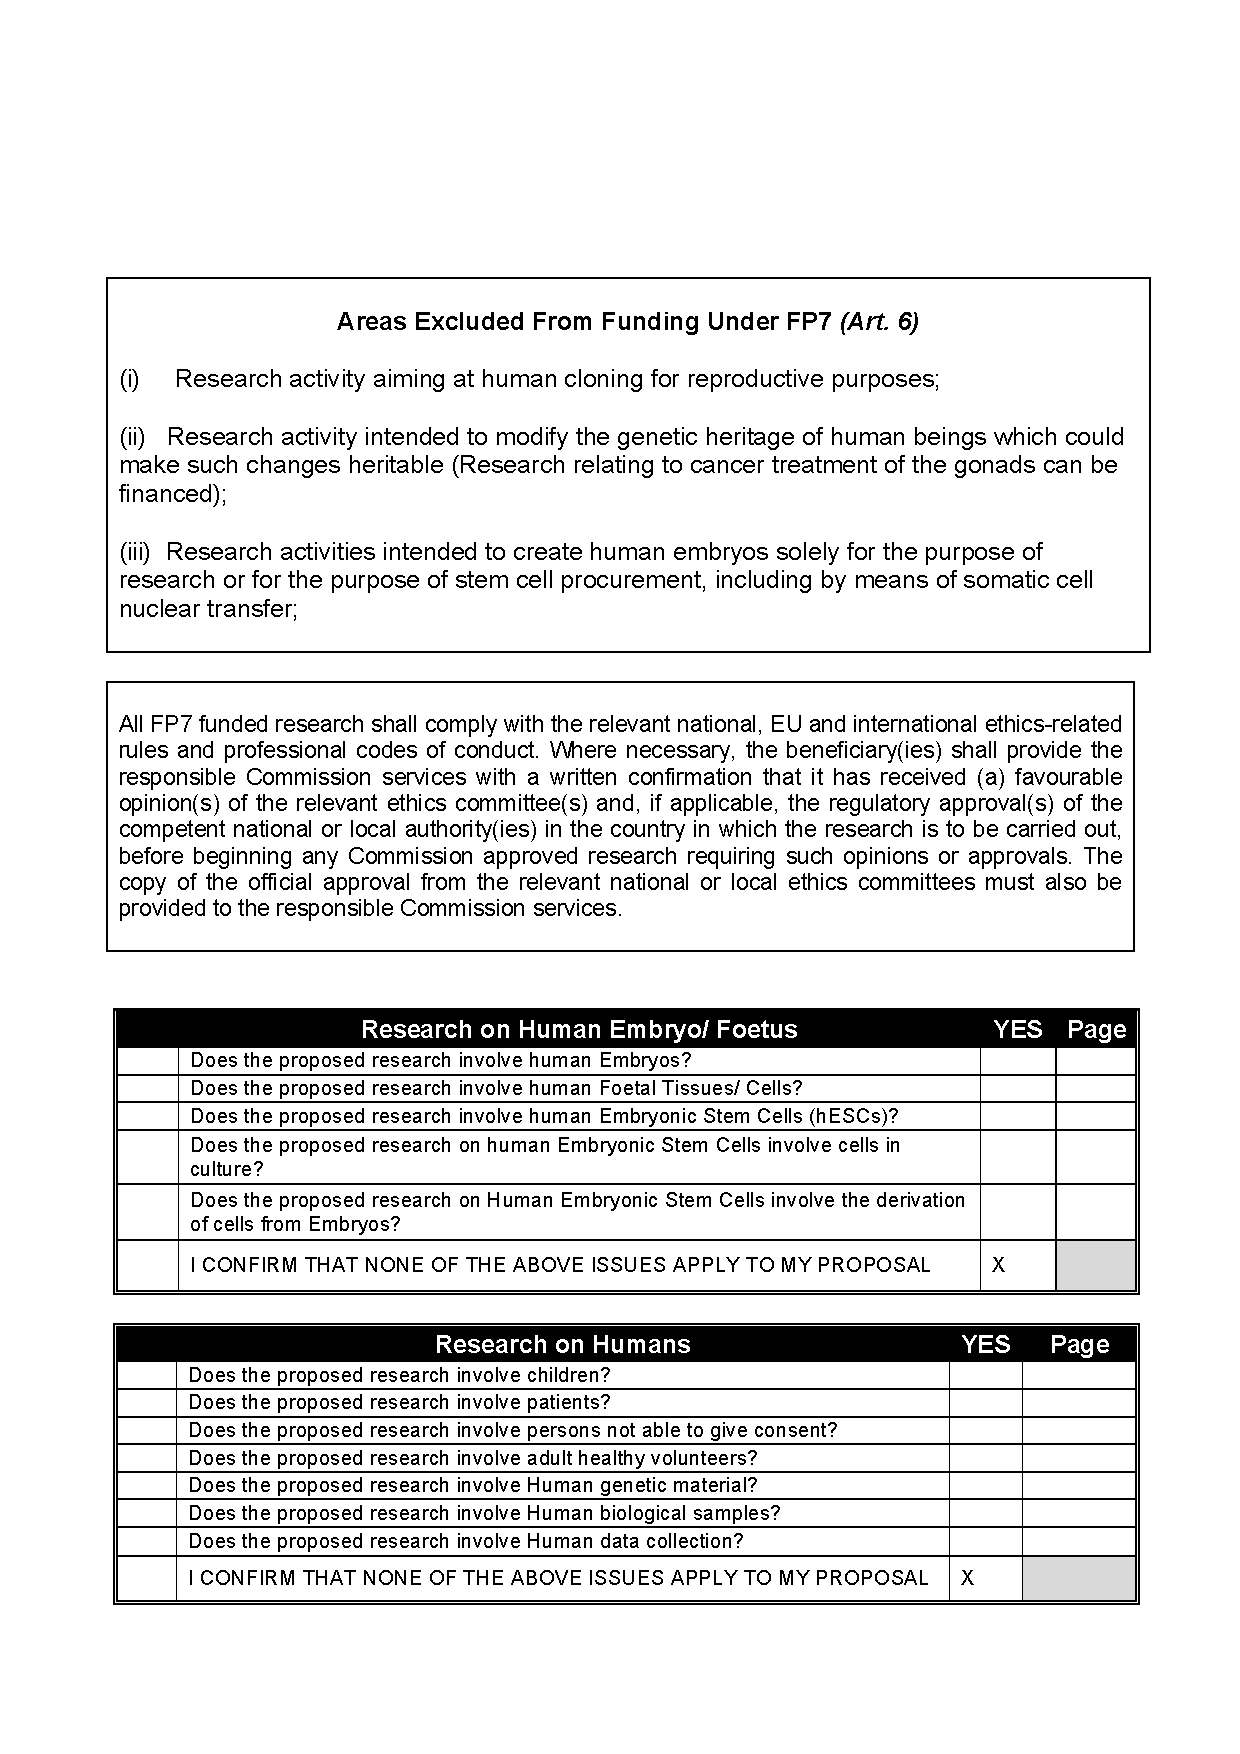
\includegraphics[width=\textwidth]{ethics1}
\end{center}

\newpage

%\mbox{}\vspace{-5mm}

\begin{center}
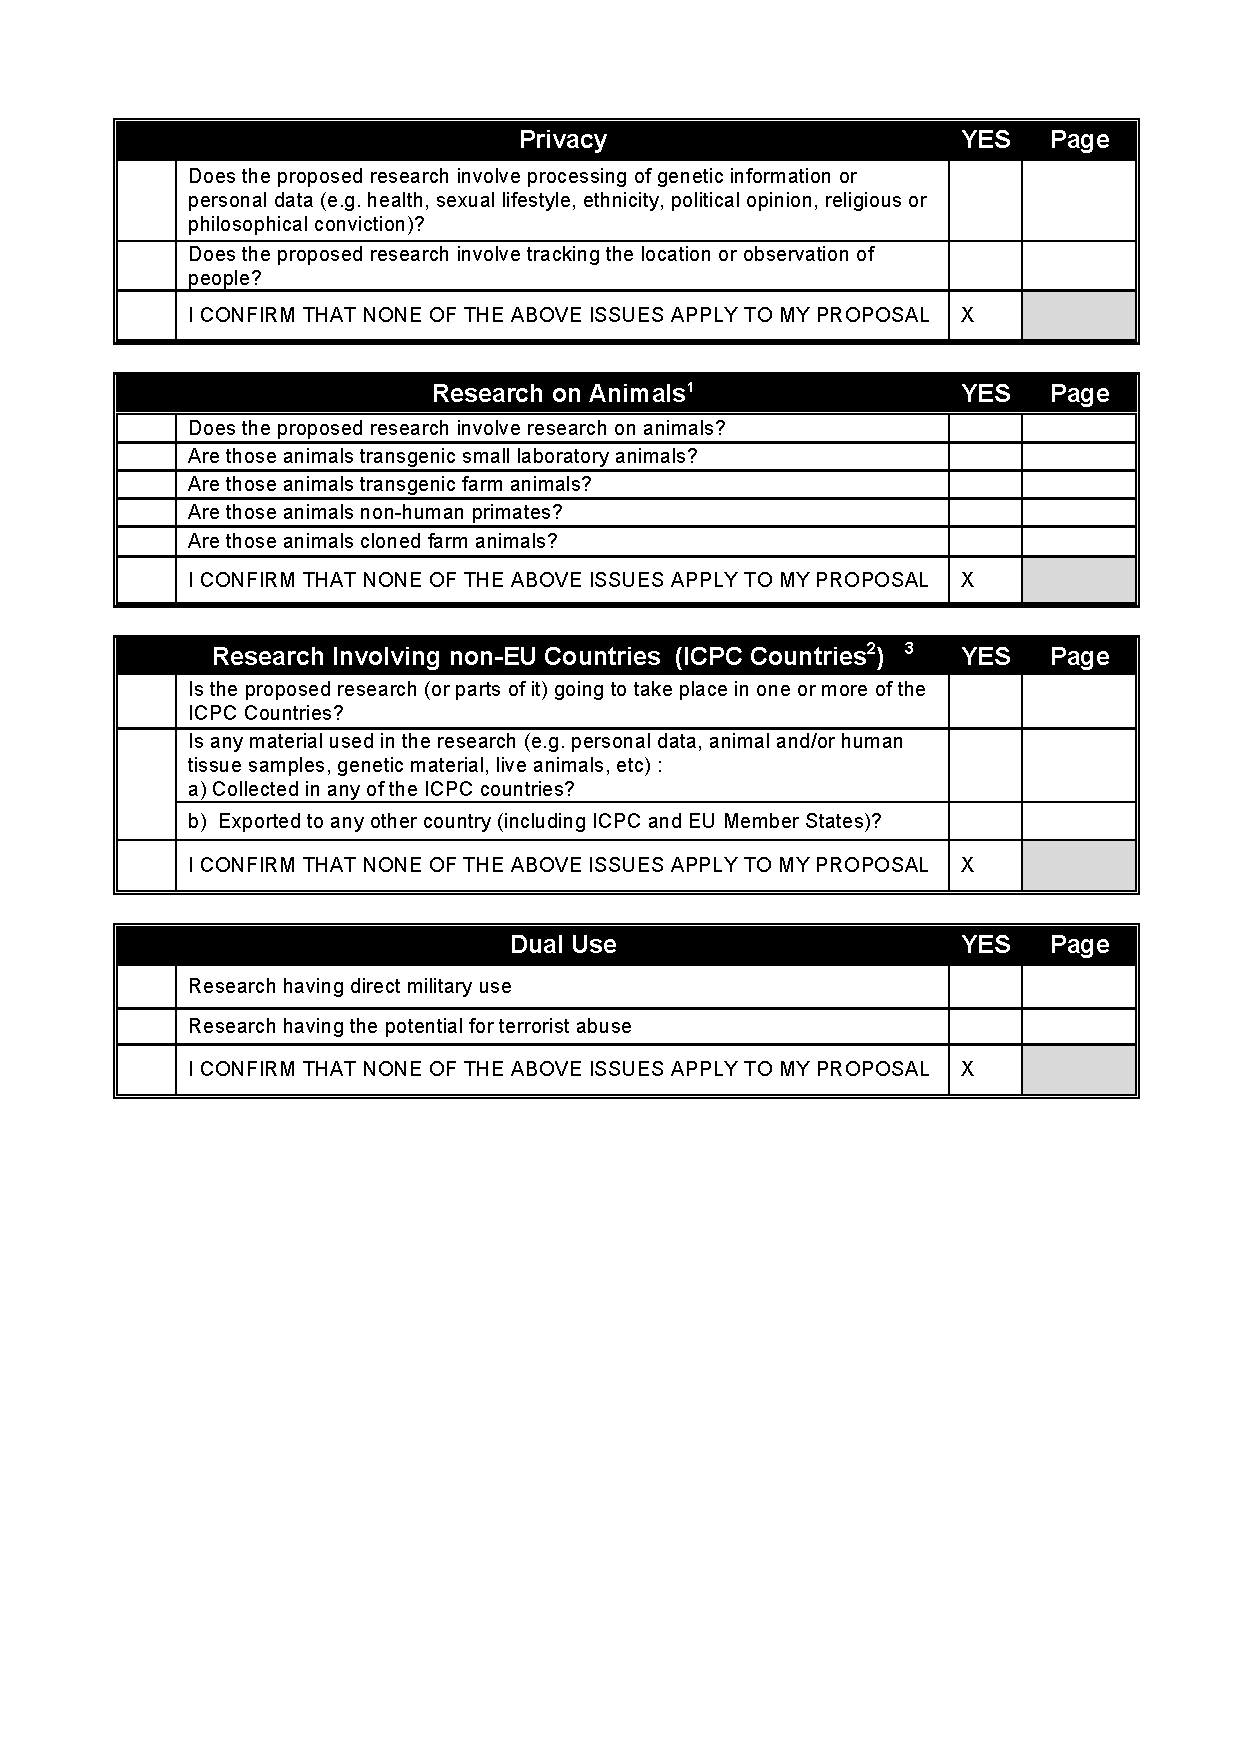
\includegraphics[width=\textwidth]{ethics3}
\end{center}


\end{document}
